% ==========================================
% BAB VI EVALUASI
% ==========================================
\cleardoublepage
\chapter{EVALUASI}
\label{chap:evaluasi}

Bab ini merupakan pelaksanaan fase demonstrasi dan evaluasi dalam metodologi \textit{Design Science Research} yang telah diuraikan pada Bab I. Setelah sistem pemantauan sampah berbasis \textit{Internet of Things} dirancang dan diimplementasikan pada Bab IV dan V, tahap selanjutnya adalah mendemonstrasikan sistem di lapangan, mengevaluasi pemenuhannya terhadap kebutuhan yang telah ditetapkan, dan menganalisis data yang dikumpulkan untuk menjawab rumusan masalah penelitian.

% ============================================================
\section{Metode Evaluasi}
\label{sec:metode-evaluasi}
% ============================================================

Evaluasi sistem pemantauan sampah berbasis \textit{Internet of Things} dilakukan secara sistematis melalui beberapa skenario yang masing-masing dirancang untuk menjawab rumusan masalah yang telah ditetapkan pada Bab I. Sebelum menjelaskan skenario evaluasi, subbab ini terlebih dahulu mendeskripsikan konfigurasi sistem dan lingkungan pengujian yang digunakan selama periode evaluasi.

\subsection{Konfigurasi Pengujian Sistem}

Pengujian sistem dilakukan dengan mengoperasikan tiga unit perangkat \textit{Smart Waste Bin} di Lantai 4 Gedung Labtek VIII Institut Teknologi Bandung. Perangkat ditempatkan di area koridor depan Laboratorium IoT. Pemilihan lokasi ini didasarkan pada beberapa pertimbangan.

\begin{enumerate}
  \item Penempatan tiga unit tempat sampah berukuran besar di area umum gedung memerlukan proses perizinan yang panjang. Area depan Laboratorium IoT memungkinkan proses perizinan yang lebih sederhana dengan dukungan dari pengelola laboratorium.
  \item Peneliti sering beraktivitas di Laboratorium IoT, sehingga memudahkan \textit{monitoring} rutin dan \textit{maintenance} perangkat jika diperlukan.
  \item Meskipun berada di ujung lantai, area ini tetap dilalui oleh pengguna gedung dan memiliki aktivitas pembuangan sampah yang dapat diobservasi.
\end{enumerate}

Setiap unit \textit{smart waste bin} diberi kode warna sesuai dengan jenis sampah yang ditampung sebagaimana disajikan pada Tabel \ref{tab:detail-unit-swb}.

% Konten pendek & seragam → tabular + \centering
\begin{table}[H]
  \caption{Detail Unit \textit{Smart Waste Bin}}
  \label{tab:detail-unit-swb}
  \centering
  \begin{tabular}{| l | l | l | l |}
    \hline
    \textbf{Sensor ID} & \textbf{Kode Warna} & \textbf{Jenis Sampah} & \textbf{MQTT \textit{Topic}} \\
    \hline
    1 & Hijau  & Organik   & \texttt{wp2/basic\_01} \\
    \hline
    2 & Kuning & Anorganik & \texttt{wp2/basic\_02} \\
    \hline
    3 & Hitam  & Residu    & \texttt{wp2/basic\_03} \\
    \hline
  \end{tabular}
\end{table}

Konfigurasi pengujian mencakup seluruh komponen sistem dari \textit{Perception Layer} hingga \textit{Application Layer}. Tabel \ref{tab:konfigurasi-lingkungan} menyajikan konfigurasi lingkungan pengujian secara keseluruhan.

% Kolom kanan perlu wrap → tabularx + X
\begin{table}[H]
  \caption{Konfigurasi Lingkungan Pengujian}
  \label{tab:konfigurasi-lingkungan}
  \begin{tabularx}{\textwidth}{| l | X |}
    \hline
    \textbf{Aspek} & \textbf{Spesifikasi} \\
    \hline
    Lokasi & Lantai 4, Gedung Labtek VIII ITB \\
    \hline
    Area Penempatan & Koridor depan Laboratorium IoT \\
    \hline
    Jumlah Perangkat & 3 unit \\
    \hline
    Periode Pengumpulan Data & 24 Desember 2025 -- 29 Januari 2026 \\
    \hline
    Interval Pengiriman Data & $\pm$2,5 jam \\
    \hline
    Konektivitas & GSM/GPRS (SIM800L) \\
    \hline
    \textit{Database} & Supabase PostgreSQL \\
    \hline
    \textit{Dashboard} & Next.js pada Vercel \\
    \hline
  \end{tabularx}
\end{table}

\subsection{Skenario Evaluasi}

Skenario evaluasi dirancang untuk menjawab setiap rumusan masalah yang telah ditetapkan pada Bab I. Tabel \ref{tab:mapping-skenario} menyajikan \textit{mapping} antara rumusan masalah, skenario evaluasi, dan tujuan evaluasi.

% Semua kolom berisi teks panjang → tabularx + X
\begin{table}[H]
  \caption{\textit{Mapping} Rumusan Masalah dengan Skenario Evaluasi}
  \label{tab:mapping-skenario}
  \begin{tabularx}{\textwidth}{| l | X | X | X |}
    \hline
    \textbf{ID} & \textbf{Rumusan Masalah} & \textbf{Skenario Evaluasi} & \textbf{Tujuan Evaluasi} \\
    \hline
    RM-1 & Rancangan dan implementasi sistem pemantauan sampah berbasis \textit{Internet of Things} (IoT) yang mampu mengumpulkan data secara periodik dan terstruktur & SE-01: Evaluasi Fungsionalitas Sistem & Memverifikasi fungsi sistem berjalan sesuai rancangan \\
    \hline
    RM-1 & & SE-02: Evaluasi Pengumpulan Data & Mengukur keberhasilan pengumpulan data periodik \\
    \hline
    RM-1 & & SE-04: Evaluasi Adaptasi \textit{Firmware} & Mengevaluasi efektivitas adaptasi \textit{firmware} terhadap keandalan sistem \\
    \hline
    RM-2 & Pola pembuangan sampah yang dapat diidentifikasi berdasarkan data sistem dan validasinya terhadap observasi lapangan & SE-03: Analisis Pola Pembuangan & Mengidentifikasi pola temporal dan validasi lapangan \\
    \hline
  \end{tabularx}
\end{table}

\subsection{Metode Analisis Data}
\label{sec:metode-analisis-data}

Untuk menjawab RM-2, data yang terkumpul dianalisis menggunakan kombinasi metode analisis statistik deskriptif dan analisis temporal. Metode analisis ditetapkan terlebih dahulu sebelum pelaksanaan analisis agar proses identifikasi pola bersifat sistematis dan dapat ditelusuri. Tahapan dan metode analisis yang digunakan adalah sebagai berikut:

\begin{enumerate}
    \item \textbf{Praproses dan Pembersihan Data}

    Data mentah hasil pengumpulan terlebih dahulu disaring untuk membuang data kotor (\textit{dirty data}) yang melanggar batas fisik yang valid, seperti nilai \textit{fillLevel} di luar rentang 0--100\% atau nilai baterai yang tidak wajar. Kriteria pembersihan ditetapkan berdasarkan batas operasional yang mustahil dicapai secara fisik, sehingga tidak ada data valid yang terbuang.

    \item \textbf{Analisis Statistik Deskriptif}

    Statistik deskriptif (nilai rata-rata, standar deviasi, nilai minimum dan maksimum, serta distribusi) dihitung untuk setiap sensor guna memberikan gambaran umum karakteristik data yang terkumpul, termasuk sebaran \textit{fillLevel} dan profil konsumsi daya.

    \item \textbf{Analisis Delta (Deteksi \textit{Event} Penambahan)}

    Karena fokus analisis adalah aktivitas pembuangan, dilakukan analisis delta, yaitu menghitung selisih nilai \textit{fillLevel} antar pembacaan berurutan. Selisih positif yang melampaui ambang tertentu diidentifikasi sebagai \textit{event} penambahan sampah. Pendekatan berbasis \textit{event} ini dipilih karena lebih relevan untuk menangkap perilaku pembuangan dibandingkan nilai \textit{fillLevel} absolut.

    \item \textbf{Analisis Temporal}

    \textit{Event} penambahan yang teridentifikasi kemudian dipetakan terhadap dimensi waktu (jam, hari, hari kerja vs akhir pekan, serta hari libur) untuk mengidentifikasi pola temporal, seperti jam puncak (\textit{peak hour}) dan rentang jam aktif.

    \item \textbf{Analisis Komparatif Antar Jenis Sampah}

    Distribusi \textit{event} dan kontribusi volume dibandingkan antar tiga jenis sampah (organik, anorganik, residu) untuk mengidentifikasi karakteristik dominasi jenis sampah.

    \item \textbf{Validasi terhadap Observasi Lapangan}

    Pola yang teridentifikasi dari data divalidasi kewajarannya melalui observasi langsung di lokasi penelitian, untuk memastikan pola yang ditemukan konsisten dengan kondisi aktual aktivitas di lapangan.
\end{enumerate}

Perlu ditegaskan bahwa proses analisis ini dilakukan oleh peneliti terhadap data yang telah dikumpulkan oleh sistem. Sistem berperan sebagai instrumen pengumpul dan penyaji data, sedangkan identifikasi pola merupakan hasil analisis yang dilakukan secara terpisah dari operasional sistem.

% ============================================================
\section{Hasil Evaluasi}
\label{sec:hasil-evaluasi}
% ============================================================

Bagian ini menyajikan hasil evaluasi untuk setiap skenario yang telah dirancang pada Subbab \ref{sec:metode-evaluasi}. Setiap skenario dilengkapi dengan metodologi pengujian, hasil pengujian, dan kesimpulan yang menjawab rumusan masalah terkait.

\subsection{Hasil Evaluasi Fungsionalitas Sistem (SE-01)}

Skenario SE-01 mengevaluasi fungsionalitas seluruh komponen sistem pemantauan sampah berbasis \textit{Internet of Things} untuk memverifikasi bahwa arsitektur dan mekanisme berfungsi sesuai dengan desain pada Bab IV. Pengujian fungsionalitas dilakukan dengan metode \textit{black-box testing} pada setiap \textit{layer} arsitektur IoT.

Tabel \ref{tab:pengujian-fungsionalitas} menyajikan komponen, aspek pengujian, dan kriteria keberhasilan untuk setiap \textit{layer}.

% Aspek & kriteria perlu wrap → tabularx + X
\begin{table}[H]
  \caption{Pengujian Fungsionalitas Sistem}
  \label{tab:pengujian-fungsionalitas}
  \begin{tabularx}{\textwidth}{| l | l | X | X |}
    \hline
    \textbf{\textit{Layer}} & \textbf{Komponen} & \textbf{Aspek Pengujian} & \textbf{Kriteria Keberhasilan} \\
    \hline
    \textit{Perception} & VL53L0X & Pengukuran jarak objek & Persentase \textit{fillLevel} sesuai dengan persentase aktual \\
    \hline
    \textit{Perception} & INA219 & \textit{Monitoring} tegangan dan arus & Nilai dalam \textit{range} operasional normal; kegagalan $\leq$1 hari berturut-turut \\
    \hline
    \textit{Network} & SIM800L & Koneksi GPRS ke jaringan & Berhasil terhubung ke APN \textit{operator} \\
    \hline
    \textit{Network} & MQTT & \textit{Publish} data ke \textit{broker} & Data terkirim dengan format valid \\
    \hline
    \textit{Middleware} & Node-RED & \textit{Response endpoint} & Status 200 dengan data valid \\
    \hline
    \textit{Application} & \textit{Dashboard} & \textit{Rendering} komponen UI & Data ditampilkan dengan benar dan lengkap \\
    \hline
    \textit{Application} & Supabase & \textit{Insert} dan \textit{query} data & Data tersimpan dengan benar \\
    \hline
  \end{tabularx}
\end{table}

\subsubsection{Hasil Pengujian \textit{Perception Layer}}

Pengujian sensor VL53L0X dilakukan dengan membandingkan pembacaan sensor dengan pengukuran manual menggunakan meteran pada berbagai jarak, sebanyak 5 kali untuk setiap titik jarak. Tabel \ref{tab:hasil-vlx} menyajikan hasilnya.

% 3 kolom medium → tabularx + X merata
\begin{table}[H]
  \caption{Hasil Pengujian Sensor VL53L0X}
  \label{tab:hasil-vlx}
  \begin{tabularx}{\textwidth}{| X | X | X |}
    \hline
    \textbf{Jarak Aktual (cm, \textit{fillLevel} \%)} & \textbf{Pembacaan Sensor (\textit{raw})} & \textbf{Pembacaan Sensor (\textit{fillLevel})} \\
    \hline
    100 ($\sim$0\%)  & Sensor 1--3: $>$900   & Sensor 1--3: 0\%   \\
    \hline
    80 ($\sim$20\%)  & Sensor 1--3: 700--799 & Sensor 1--3: 20\%  \\
    \hline
    60 ($\sim$40\%)  & Sensor 1--3: 500--599 & Sensor 1--3: 40\%  \\
    \hline
    20 ($\sim$80\%)  & Sensor 1--3: 100--199 & Sensor 1--3: 80\%  \\
    \hline
    0 ($\sim$100\%)  & Sensor 1--3: 0--99    & Sensor 1--3: 100\% \\
    \hline
  \end{tabularx}
\end{table}

Penggunaan tipe data integer menyebabkan pembulatan (\textit{truncation}) yang memberikan efek stabilisasi pada indikator \textit{dashboard} agar tidak terlalu fluktuatif. Hasil pengujian menunjukkan kesesuaian yang tinggi antara pengukuran manual dengan \textit{output} sistem.

Pengujian sensor INA219 dilakukan selama periode pengumpulan data untuk memverifikasi keandalan pembacaan tegangan, arus, dan daya. Tabel \ref{tab:hasil-ina219} menyajikan hasilnya.

% 6 kolom pendek → tabular + \centering
\begin{table}[H]
  \caption{Hasil Pengujian Sensor INA219}
  \label{tab:hasil-ina219}
  \centering
  \begin{tabular}{| l | l | l | l | l | l |}
    \hline
    \textbf{Sensor} & \textbf{Jenis} & \textbf{Tegangan (V)} & \textbf{Arus (mA)} & \textbf{Daya (mW)} & \textbf{Status} \\
    \hline
    1 & Organik   & 7,30--7,50 & 110--140 & 803--1.050   & OK \\
    \hline
    2 & Anorganik & 7,10--7,45 & 110--135 & 781--1.006   & OK \\
    \hline
    3 & Residu    & 6,90--7,50 & 210--235 & 1.449--1.763 & FAILED \\
    \hline
  \end{tabular}
\end{table}

Sensor 3 (Residu) menunjukkan konsumsi arus hampir dua kali lipat (210--235 mA) dibandingkan sensor lainnya (110--140 mA). Sensor 3 juga mengalami kegagalan INA219 selama 4 hari berturut-turut (11--14 Januari 2026), melebihi batas kriteria 1 hari berturut-turut. Kegagalan ini bertepatan dengan gangguan kabel I2C yang juga menyebabkan kegagalan VL53L0X secara bersamaan. Setelah perbaikan kabel, pembacaan kembali normal.

\subsubsection{Hasil Pengujian \textit{Network Layer}}

Pengujian \textit{Network Layer} dilakukan sebelum pemasangan perangkat dengan memverifikasi \textit{output debug} pada \textit{Serial Monitor}. Tabel \ref{tab:hasil-gprs} menyajikan hasil pengujian modem GPRS.

% Kolom tengah perlu wrap → tabularx
\begin{table}[H]
  \caption{Hasil Pengujian Modem GPRS}
  \label{tab:hasil-gprs}
  \begin{tabularx}{\textwidth}{| l | X | l |}
    \hline
    \textbf{Tahap} & \textbf{\textit{Output Serial Monitor}} & \textbf{Status} \\
    \hline
    Inisialisasi Modem  & Initializing modem\ldots           & OK \\
    \hline
    Info Modem          & Modem Info: SIM800 R14.18          & OK \\
    \hline
    Registrasi Jaringan & Waiting for network\ldots success  & OK \\
    \hline
    Koneksi APN         & Connecting to M2MINTERNET\ldots success & OK \\
    \hline
    Status GPRS         & GPRS connected                     & OK \\
    \hline
  \end{tabularx}
\end{table}

Pengujian MQTT dilakukan dalam dua tahap: menggunakan \textit{listener} lokal untuk memverifikasi data terkirim, kemudian menggunakan Node-RED sebagai \textit{subscriber}. Tabel \ref{tab:hasil-mqtt} menyajikan hasilnya.

% Kolom tengah perlu wrap → tabularx
\begin{table}[H]
  \caption{Hasil Pengujian MQTT}
  \label{tab:hasil-mqtt}
  \begin{tabularx}{\textwidth}{| l | X | l |}
    \hline
    \textbf{Tahap} & \textbf{Hasil} & \textbf{Status} \\
    \hline
    Koneksi ke \textit{Broker}   & Connecting to 38.47.176.109\ldots success & OK \\
    \hline
    Test \textit{Listener} Lokal & Data JSON diterima pada \textit{topic} \texttt{wp2/basic\_01}, \texttt{\_02}, \texttt{\_03} & OK \\
    \hline
    Test ke Node-RED             & Node-RED menerima dan mem-\textit{parse} data JSON dengan benar & OK \\
    \hline
    Format \textit{Payload}      & JSON valid dengan seluruh \textit{field} yang diperlukan & OK \\
    \hline
  \end{tabularx}
\end{table}

\subsubsection{Hasil Pengujian \textit{Middleware Layer} dan \textit{Application Layer}}

Pengujian \textit{Middleware Layer} memastikan setiap \textit{payload} MQTT berhasil ditangkap, di-\textit{parse}, dan disimpan ke \textit{database} tanpa \textit{data loss} atau \textit{corrupt}. Tabel \ref{tab:hasil-nodered} menyajikan hasilnya.

% Dua kolom pertama perlu wrap → tabularx
\begin{table}[H]
  \caption{Hasil Pengujian Node-RED}
  \label{tab:hasil-nodered}
  \begin{tabularx}{\textwidth}{| X | X | l |}
    \hline
    \textbf{Aspek Pengujian} & \textbf{Hasil} & \textbf{Status} \\
    \hline
    \textit{Subscribe} MQTT    & Berhasil \textit{subscribe} ke ketiga \textit{topic} & OK \\
    \hline
    \textit{Parsing} JSON      & Data di-\textit{parse} dengan benar menggunakan JSON \textit{node} & OK \\
    \hline
    \textit{Insert} ke Supabase & Data diteruskan ke Supabase melalui HTTP \textit{request} & OK \\
    \hline
    \textit{Data Integrity}    & Tidak ada data \textit{corrupt} atau duplikat & OK \\
    \hline
    \textit{Query Performance} & \textit{Response time} $<$500ms untuk \textit{query} 1 minggu & OK \\
    \hline
  \end{tabularx}
\end{table}

Pengujian API \textit{endpoint} dilakukan dengan \textit{request} HTTP GET menggunakan berbagai parameter \textit{filter}. Tabel \ref{tab:hasil-api} menyajikan hasilnya.

% Kolom endpoint panjang → tabularx, sisanya pendek → l
\begin{table}[H]
  \caption{Hasil Pengujian API \textit{Dashboard}}
  \label{tab:hasil-api}
  \begin{tabularx}{\textwidth}{| X | l | l | l | l |}
    \hline
    \textbf{\textit{Endpoint}} & \textbf{Method} & \textbf{Expected} & \textbf{Aktual} & \textbf{Status} \\
    \hline
    \texttt{/api/sensor-data}                   & GET & 200, array             & 200 & OK \\
    \hline
    \texttt{/api/sensor-data?sensorId=1}        & GET & 200, \textit{filtered} & 200 & OK \\
    \hline
    \texttt{/api/sensor-data?sensorId=2}        & GET & 200, \textit{filtered} & 200 & OK \\
    \hline
    \texttt{/api/sensor-data?sensorId=3}        & GET & 200, \textit{filtered} & 200 & OK \\
    \hline
    \texttt{/api/sensor-data?timerange=24h}     & GET & 200, 24h data          & 200 & OK \\
    \hline
    \texttt{/api/sensor-data?timerange=7d}      & GET & 200, 7d data           & 200 & OK \\
    \hline
  \end{tabularx}
\end{table}

Pengujian antarmuka \textit{dashboard} dilakukan secara \textit{end-to-end} untuk memverifikasi visualisasi dan fitur interaktif. Tabel \ref{tab:hasil-ui} menyajikan hasilnya.

% Kolom tengah perlu wrap → tabularx
\begin{table}[H]
  \caption{Hasil Pengujian Komponen \textit{Dashboard}}
  \label{tab:hasil-ui}
  \begin{tabularx}{\textwidth}{| l | X | l |}
    \hline
    \textbf{Komponen} & \textbf{Aspek Pengujian} & \textbf{Hasil} \\
    \hline
    \textit{Header Section}   & Menampilkan judul, tombol \textit{refresh}, \textit{last update} & Sesuai \\
    \hline
    \textit{Sensor Cards}     & Menampilkan status 3 sensor dengan warna \textit{threshold} & Sesuai \\
    \hline
    \textit{Fill Level} Bar   & \textit{Progress bar} sesuai persentase \textit{fillLevel} & Sesuai \\
    \hline
    \textit{Control Panel}    & \textit{Filter} sensor dan \textit{time range} berfungsi & Sesuai \\
    \hline
    Chart \textit{Fill Level} & \textit{Line chart} menampilkan tren \textit{fillLevel} & Sesuai \\
    \hline
    Chart \textit{Battery}    & \textit{Dual-axis chart} baterai dan \textit{power consumption} & Sesuai \\
    \hline
    \textit{Auto-refresh}     & Data ter-\textit{update} setiap 30 detik & Sesuai \\
    \hline
  \end{tabularx}
\end{table}

Seluruh komponen sistem dari \textit{Perception Layer} hingga \textit{Application Layer} berfungsi sesuai dengan desain. Hasil pengujian ini menjawab RM-1 terkait komponen, arsitektur, dan mekanisme sistem pemantauan sampah berbasis \textit{Internet of Things} (IoT).

\subsection{Hasil Evaluasi Pengumpulan Data (SE-02)}

Skenario SE-02 mengevaluasi keberhasilan dan konsistensi pengumpulan data secara periodik selama periode observasi.

\subsubsection{Periode Pengumpulan Data}

Tabel \ref{tab:detail-pengumpulan} menyajikan detail periode pengumpulan data.

% Kolom kanan perlu wrap → tabularx
\begin{table}[H]
  \caption{Detail Pengumpulan Data}
  \label{tab:detail-pengumpulan}
  \begin{tabularx}{\textwidth}{| l | X |}
    \hline
    \textbf{Aspek} & \textbf{Nilai} \\
    \hline
    Tanggal mulai & 24 Desember 2025 \\
    \hline
    Tanggal selesai & 29 Januari 2026 \\
    \hline
    Total durasi & 37 hari \\
    \hline
    Hari kerja (Senin--Jumat) & 24 hari \\
    \hline
    \textit{Weekend} (Sabtu--Minggu) & 10 hari \\
    \hline
    Hari libur nasional & 3 hari (25--26 Des 2025, 1 Jan 2026) \\
    \hline
    Target interval pengiriman & $\pm$2,5 jam (\texttt{TIME\_TO\_SLEEP} = 150 menit) \\
    \hline
  \end{tabularx}
\end{table}

\subsubsection{Volume Data Terkumpul}

Tabel \ref{tab:volume-data} menyajikan jumlah data yang berhasil dikumpulkan dari setiap sensor.

% 6 kolom pendek → tabular + \centering
\begin{table}[H]
  \caption{Jumlah Data Terkumpul per Sensor}
  \label{tab:volume-data}
  \centering
  \begin{tabular}{| l | l | l | l | l | l |}
    \hline
    \textbf{Sensor} & \textbf{Jenis} & \textbf{\textit{Records}} & \textbf{Target} & \textbf{Pencapaian} & \textbf{Status} \\
    \hline
    1     & Organik   & 289 & 296 & 97,6\% & OK \\
    \hline
    2     & Anorganik & 290 & 296 & 98,0\% & OK \\
    \hline
    3     & Residu    & 237 & 296 & 80,0\% & Sebagian OK \\
    \hline
    Total & --        & 816 & 888 & 91,9\% & -- \\
    \hline
  \end{tabular}
\end{table}

Target 296 \textit{records} per sensor diperoleh dari 37 hari $\times$ 8 \textit{records}/hari (interval 3 jam). Sensor 1 (Organik) dan Sensor 2 (Anorganik) mencapai target mendekati 100\%. Sensor 3 (Residu) mencapai 80,0\% yang lebih rendah karena konsumsi daya lebih tinggi (210--235 mA vs 110--140 mA) sehingga baterai lebih cepat habis. Dari 816 \textit{records} yang terkirim, 805 \textit{records} dinyatakan valid setelah \textit{filtering} data kotor.

\subsubsection{Konsistensi Interval Pengiriman}

Tabel \ref{tab:statistik-interval} menyajikan statistik interval pengiriman data untuk setiap sensor.

% 5 kolom pendek-medium → tabular + \centering
\begin{table}[H]
  \caption{Statistik Interval Pengiriman Data}
  \label{tab:statistik-interval}
  \centering
  \begin{tabular}{| l | l | l | l | l |}
    \hline
    \textbf{Sensor} & \textbf{Rata-rata} & \textbf{Minimum} & \textbf{Maksimum} & \textbf{Std Dev} \\
    \hline
    1 & 2 jam 24 menit & 35 menit & 4 jam 58 menit & 25 menit \\
    \hline
    2 & 2 jam 24 menit & 22 menit & 5 jam 22 menit & 31 menit \\
    \hline
    3 & 2 jam 21 menit & 2 menit* & 4 jam 57 menit & 38 menit \\
    \hline
  \end{tabular}
\end{table}

*Nilai minimum sangat kecil merupakan indikasi \textit{retry} pengiriman setelah koneksi gagal, bukan interval reguler. Rata-rata interval $\pm$144 menit ($\approx$2 jam 24 menit) mendekati target \texttt{TIME\_TO\_SLEEP} = 150 menit.

\subsubsection{Analisis \textit{Data Loss} dan Data Kotor}

Tabel \ref{tab:analisis-dataloss} menyajikan analisis penyebab \textit{data loss} selama periode pengumpulan.

% Kolom pertama & terakhir perlu wrap → tabularx
\begin{table}[H]
  \caption{Penyebab \textit{Data Loss} dan Data Kotor}
  \label{tab:analisis-dataloss}
  \begin{tabularx}{\textwidth}{| X | l | l | X |}
    \hline
    \textbf{Kategori} & \textbf{Jumlah} & \textbf{\%} & \textbf{Penyebab} \\
    \hline
    Data sukses terkirim & 816 & 91,9\% & -- \\
    \hline
    Baterai habis/bocor & 64 & 7,2\% & \textit{Deep sleep} karena baterai habis; 4 baterai bocor (mati total), terutama pada Sensor 3 \\
    \hline
    MQTT \textit{broker} \textit{down} & 8 & 0,9\% & \textit{Broker} dimatikan pihak ketiga; pengumpulan dihentikan 29 Januari 2026 \\
    \hline
    \textbf{Total \textit{data loss}} & \textbf{72} & \textbf{8,1\%} & Dalam batas toleransi ($<$10\%) \\
    \hline
  \end{tabularx}
\end{table}

Selain \textit{data loss}, terdapat data yang berhasil terkirim namun memiliki nilai tidak valid. Tabel \ref{tab:jenis-data-kotor} menyajikan jenis-jenis data kotor yang teridentifikasi.

% Kolom indikator & penyebab panjang → tabularx
\begin{table}[H]
  \caption{Jenis-jenis Data Kotor}
  \label{tab:jenis-data-kotor}
  \begin{tabularx}{\textwidth}{| l | l | X | X |}
    \hline
    \textbf{Jenis Anomali} & \textbf{Jumlah} & \textbf{Indikator} & \textbf{Penyebab} \\
    \hline
    \textit{Battery} 999\% & 7 & tegangan = arus = batt = 999, \textit{fillLevel} = -1, \texttt{ina219\_avail} = 0, \texttt{vl53l0x\_avail} = 0 & Kabel I2C putus total; seluruhnya dari Sensor 3 \\
    \hline
    \textit{fillLevel} = -1 atau $>$100 & 3 & \textit{fillLevel} di luar 0--100\% & VL53L0X \textit{timeout} atau \textit{error} \\
    \hline
  \end{tabularx}
\end{table}

Dari 816 \textit{records} yang terkirim, terdapat 11 \textit{record} kotor (1,3\%) yang seluruhnya berasal dari Sensor 3 (Residu), disebabkan oleh masalah kabel I2C yang konsisten dengan anomali konsumsi daya tinggi pada unit tersebut. Setelah \textit{filtering}, tersisa 805 \textit{records} bersih. Data kotor dapat diidentifikasi melalui kolom \texttt{vl53l0x\_avail} dan \texttt{ina219\_avail}.

\subsubsection{Kualitas Data Setelah \textit{Filtering}}

Tabel \ref{tab:kualitas-data} menyajikan hasil analisis kualitas data setelah \textit{filtering} berdasarkan kolom \textit{availability} sensor.

% Kolom pertama panjang → tabularx + X
\begin{table}[H]
  \caption{Hasil Kualitas Data Setelah \textit{Filtering}}
  \label{tab:kualitas-data}
  \begin{tabularx}{\textwidth}{| X | l |}
    \hline
    \textbf{Metrik Kualitas} & \textbf{Hasil} \\
    \hline
    \multicolumn{2}{|l|}{\textit{Sebelum filter}: 816 \textit{records} \quad \textit{Setelah filter}: 805 \textit{records} (98,7\%)} \\
    \hline
    Data dengan \texttt{vl53l0x\_avail} = 1 (sensor jarak aktif) & 100\% \\
    \hline
    Data dengan \texttt{ina219\_avail} = 1 (sensor daya aktif) & 100\% \\
    \hline
    \textit{fillLevel} dalam \textit{range} valid (0--100\%) setelah \textit{filter} & 100\% \\
    \hline
    \textit{Timestamp} valid (format ISO 8601, \textit{timezone} Asia/Jakarta) & 100\% \\
    \hline
    Tidak ada duplikat (unique \textit{timestamp} + \texttt{sensor\_id}) & 100\% \\
    \hline
    \textit{Battery percentage} dalam \textit{range} valid (0--100\%) & 100\% \\
    \hline
    \texttt{sensor\_id} valid (1, 2, atau 3) & 100\% \\
    \hline
  \end{tabularx}
\end{table}

Kualitas data yang terkumpul sangat baik dengan validitas 100\% untuk semua metrik setelah \textit{filtering}. Data dengan \texttt{vl53l0x\_avail} = 0 atau \texttt{ina219\_avail} = 0 di-\textit{filter} pada tahap \textit{preprocessing} sebelum analisis pola.

\subsubsection{Distribusi Temporal Data}

Tabel \ref{tab:distribusi-jam} dan Tabel \ref{tab:distribusi-hari} menyajikan distribusi data berdasarkan waktu untuk memastikan data terdistribusi merata.

% 3 kolom pendek → tabular + \centering
\begin{table}[H]
  \caption{Jumlah \textit{Record} per Rentang Jam}
  \label{tab:distribusi-jam}
  \centering
  \begin{tabular}{| l | l | l |}
    \hline
    \textbf{Rentang Jam} & \textbf{Jumlah \textit{Records}} & \textbf{Persentase} \\
    \hline
    07:00--09:00        & 56  & 7,0\%  \\
    \hline
    09:00--12:00        & 81  & 10,1\% \\
    \hline
    12:00--14:00        & 53  & 6,6\%  \\
    \hline
    14:00--17:00        & 119 & 14,8\% \\
    \hline
    17:00--19:00        & 73  & 9,1\%  \\
    \hline
    19:00--07:00        & 423 & 52,5\% \\
    \hline
    \textbf{Total}      & \textbf{805} & \textbf{100\%} \\
    \hline
  \end{tabular}
\end{table}

% 3 kolom pendek → tabular + \centering
\begin{table}[H]
  \caption{Jumlah \textit{Record} per Hari}
  \label{tab:distribusi-hari}
  \centering
  \begin{tabular}{| l | l | l |}
    \hline
    \textbf{Hari} & \textbf{Jumlah \textit{Records}} & \textbf{Persentase} \\
    \hline
    Senin         & 102 & 12,7\% \\
    \hline
    Selasa        & 127 & 15,8\% \\
    \hline
    Rabu          & 153 & 19,0\% \\
    \hline
    Kamis         & 135 & 16,8\% \\
    \hline
    Jumat         & 108 & 13,4\% \\
    \hline
    Sabtu         & 91  & 11,3\% \\
    \hline
    Minggu        & 89  & 11,1\% \\
    \hline
    \textbf{Total} & \textbf{805} & \textbf{100\%} \\
    \hline
  \end{tabular}
\end{table}

Rentang 19:00--07:00 mendominasi distribusi jam (52,5\%) karena sensor mengirim data setiap $\pm$2,5 jam selama 24 jam penuh termasuk malam hari. Dari 805 \textit{records}, sebanyak 382 \textit{records} (47,5\%) berasal dari jam aktif kampus (07:00--19:00). Distribusi per hari relatif merata dengan hari kerja (Senin--Jumat) masing-masing berkontribusi 12--19\%, sedangkan Sabtu dan Minggu masing-masing 11,3\% dan 11,1\%.

\subsection{Hasil Analisis Pola Pembuangan Sampah (SE-03)}

Skenario SE-03 mengidentifikasi pola temporal pembuangan sampah berdasarkan data yang dikumpulkan dan memvalidasinya dengan observasi lapangan untuk menjawab RM-2. Analisis dilakukan menggunakan \textit{script} Python yang mencakup \textit{data cleaning}, perhitungan statistik deskriptif, dan visualisasi pola (kode sumber tersedia pada Lampiran A).

\subsubsection{Statistik Deskriptif \textit{fillLevel}}

Tabel \ref{tab:statistik-filllevel} menyajikan statistik deskriptif \textit{fillLevel} untuk setiap sensor selama periode observasi.

\begin{table}[H]
  \caption{Statistik Deskriptif \textit{fillLevel} per Sensor}
  \label{tab:statistik-filllevel}
  \centering
  \begin{tabular}{| l | l | l | l |}
    \hline
    \textbf{Statistik} & \textbf{Organik (S1)} & \textbf{Anorganik (S2)} & \textbf{Residu (S3)} \\
    \hline
    Jumlah data (n) & 289    & 290    & 226 \\
    \hline
    \textit{Mean}   & 5,3\%  & 14,4\% & 6,4\% \\
    \hline
    Median          & 0\%    & 10\%   & 10\% \\
    \hline
    Modus           & 0\%    & 0\%    & 10\% \\
    \hline
    Std Deviasi     & 5,7\%  & 13,0\% & 6,0\% \\
    \hline
    Minimum         & 0\%    & 0\%    & 0\% \\
    \hline
    Maksimum        & 20\%   & 40\%   & 20\% \\
    \hline
  \end{tabular}
\end{table}

\begin{figure}[H]
  \caption{Statistik \textit{fillLevel} per Sensor}
  \label{fig:statistik-filllevel}
  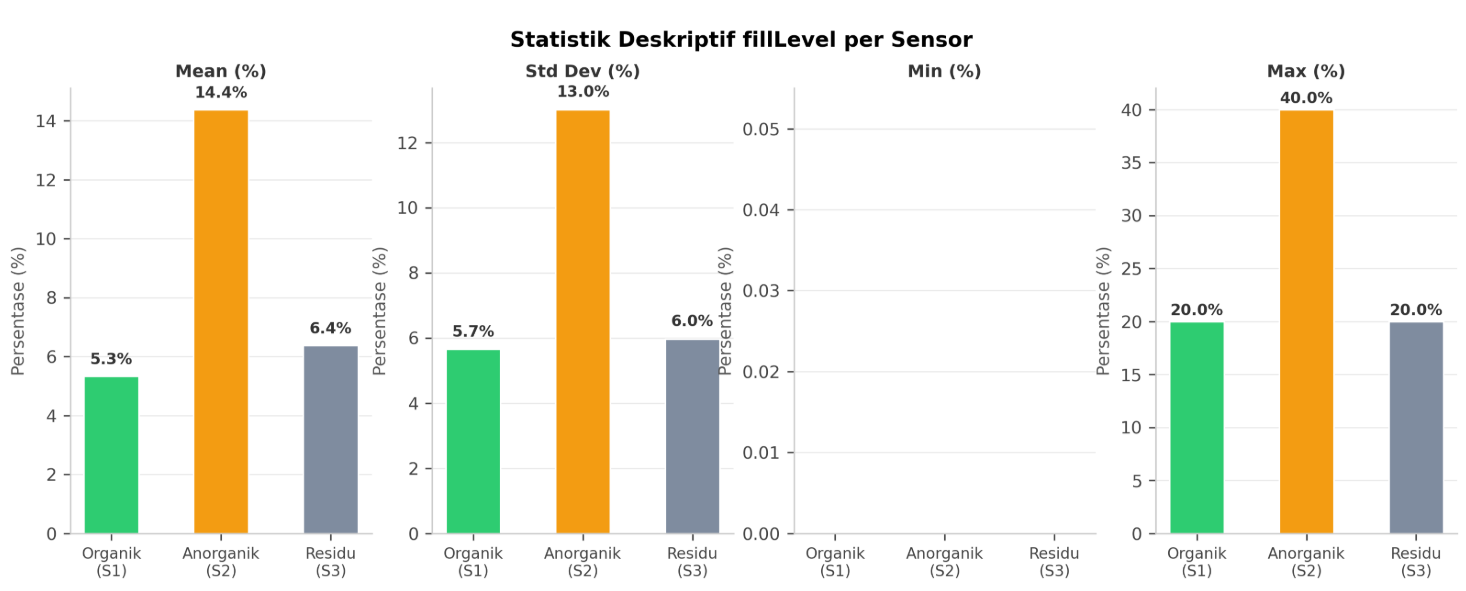
\includegraphics[width=\textwidth]{images/statistik-filllevel.png}
  % RENAME: image15.png → statistik-filllevel.png
\end{figure}

Sensor 2 (Anorganik) memiliki rata-rata \textit{fillLevel} tertinggi (14,4\%) dengan variasi terbesar (std 13,0\%), menunjukkan aktivitas pembuangan sampah anorganik paling tinggi di lokasi pengujian, sebagaimana divisualisasikan pada Gambar \ref{fig:statistik-filllevel}. Median Organik (S1) bernilai 0\% karena lebih dari separuh \textit{records} memiliki \textit{fillLevel} 0\%, mencerminkan frekuensi pengosongan yang tinggi.

\subsubsection{Distribusi \textit{fillLevel}}

Tabel \ref{tab:distribusi-filllevel} menyajikan distribusi frekuensi nilai \textit{fillLevel} pada setiap sensor.

\begin{table}[H]
  \caption{Distribusi \textit{fillLevel} per Sensor}
  \label{tab:distribusi-filllevel}
  \centering
  \begin{tabular}{| l | l | l | l |}
    \hline
    \textbf{\textit{fillLevel}} & \textbf{Organik (S1)} & \textbf{Anorganik (S2)} & \textbf{Residu (S3)} \\
    \hline
    0\%  & 145 (50,2\%) & 93 (32,1\%)  & 96 (42,5\%) \\
    \hline
    10\% & 134 (46,4\%) & 66 (22,8\%)  & 116 (51,3\%) \\
    \hline
    20\% & 10 (3,5\%)   & 69 (23,8\%)  & 14 (6,2\%) \\
    \hline
    30\% & 0 (0\%)      & 35 (12,1\%)  & 0 (0\%) \\
    \hline
    40\% & 0 (0\%)      & 27 (9,3\%)   & 0 (0\%) \\
    \hline
  \end{tabular}
\end{table}

Sampah Anorganik memiliki distribusi \textit{fillLevel} paling bervariasi dengan nilai mencapai 40\%, sedangkan Organik dan Residu didominasi oleh \textit{fillLevel} rendah (0--10\%) yang menunjukkan tempat sampah dikosongkan secara rutin.

\subsubsection{Pola Temporal Harian}

Analisis pola harian dilakukan dengan mengelompokkan rata-rata \textit{fillLevel} berdasarkan rentang jam, sebagaimana disajikan pada Tabel \ref{tab:pola-harian} dan divisualisasikan pada Gambar \ref{fig:pola-harian}. Nilai yang ditampilkan merupakan rata-rata \textit{fillLevel} kumulatif per slot waktu, bukan laju penambahan.

\begin{table}[H]
  \caption{Pola Temporal Harian}
  \label{tab:pola-harian}
  \begin{tabularx}{\textwidth}{| l | l | l | l | X |}
    \hline
    \textbf{Rentang Jam} & \textbf{Organik} & \textbf{Anorganik} & \textbf{Residu} & \textbf{Keterangan} \\
    \hline
    07:00--09:00 & 6,5\%  & 11,4\% & 5,7\%  & Awal aktivitas kampus \\
    \hline
    09:00--12:00 & 5,9\%  & 14,8\% & 8,8\%  & Jam kerja/kuliah pagi \\
    \hline
    12:00--14:00 & 7,8\%  & 13,2\% & 10,0\% & Jam makan siang \\
    \hline
    14:00--17:00 & 5,6\%  & 13,4\% & 5,7\%  & Jam kerja/kuliah sore \\
    \hline
    17:00--19:00 & 5,6\%  & 15,7\% & 5,5\%  & Akhir aktivitas \\
    \hline
    19:00--07:00 & 4,7\%  & 14,9\% & 5,8\%  & Non-aktif (malam) \\
    \hline
  \end{tabularx}
\end{table}

\begin{figure}[H]
  \caption{Distribusi \textit{fillLevel} per Rentang Jam}
  \label{fig:pola-harian}
  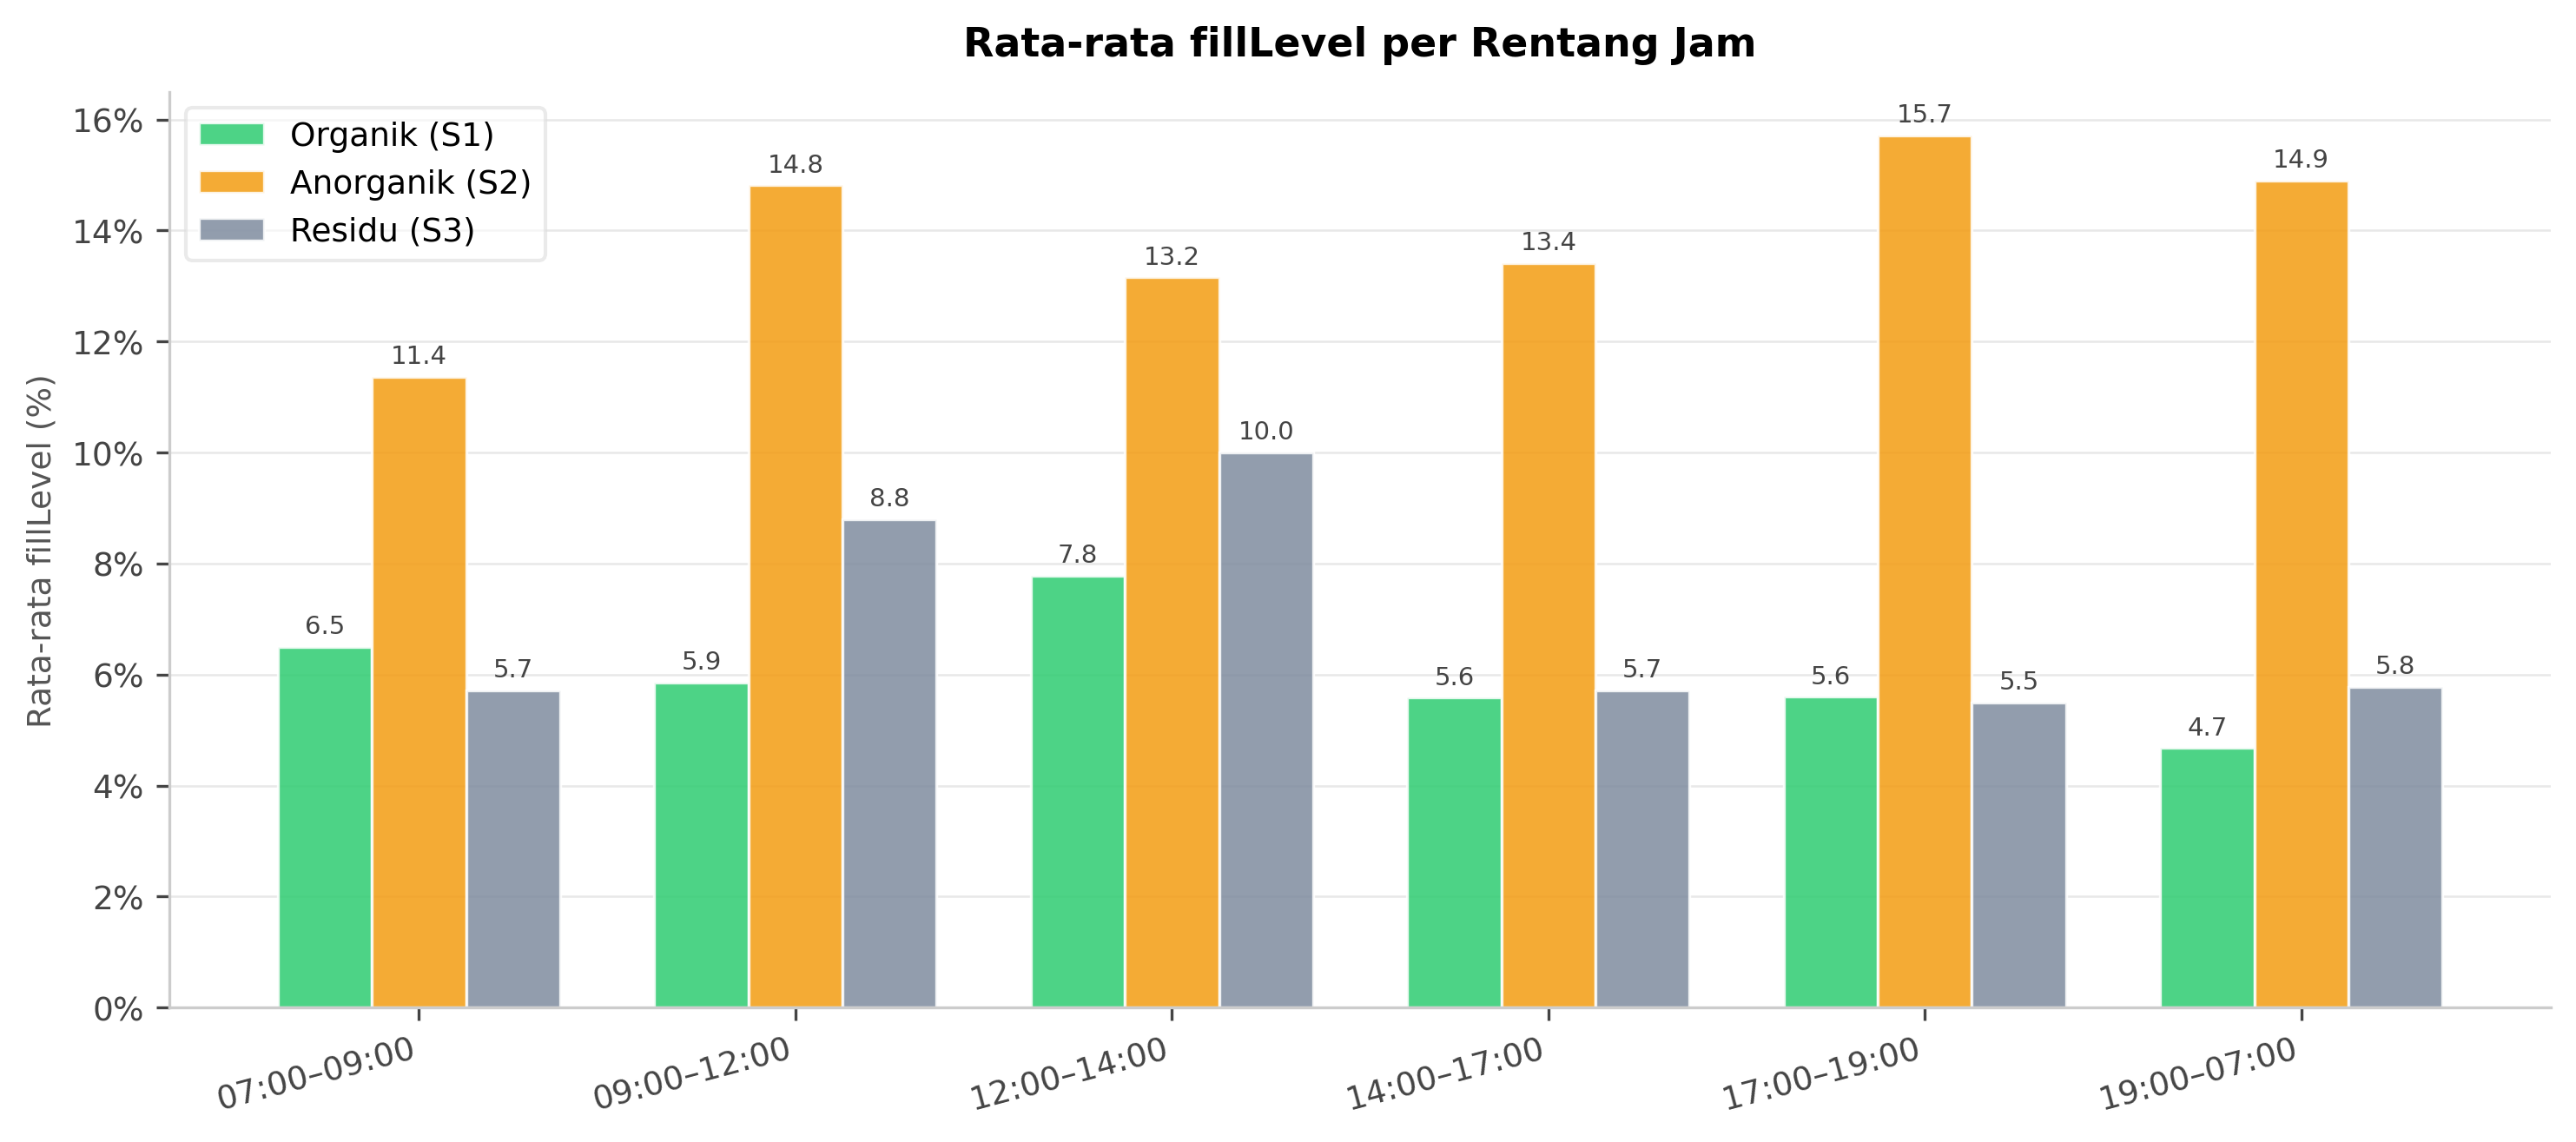
\includegraphics[width=\textwidth]{images/pola-harian.png}
  % RENAME: image16.png → pola-harian.png
\end{figure}

Nilai \textit{fillLevel} tertinggi pada S1 (Organik) dan S3 (Residu) terjadi pada rentang 12:00--14:00, konsisten dengan aktivitas makan siang. S2 (Anorganik) menunjukkan \textit{fillLevel} relatif tinggi dan merata sepanjang hari.

\subsubsection{Pola Temporal Mingguan}

Analisis pola mingguan dilakukan dengan mengelompokkan rata-rata \textit{fillLevel} berdasarkan hari, sebagaimana disajikan pada Tabel \ref{tab:pola-mingguan} dan divisualisasikan pada Gambar \ref{fig:pola-mingguan}. Nilai \textit{fillLevel} bersifat kumulatif antar pengosongan sehingga pola dipengaruhi jadwal pengosongan aktual, bukan semata aktivitas pengguna.

\begin{table}[H]
  \caption{Pola Temporal Mingguan}
  \label{tab:pola-mingguan}
  \centering
  \begin{tabular}{| l | l | l | l | l |}
    \hline
    \textbf{Hari} & \textbf{Organik} & \textbf{Anorganik} & \textbf{Residu} & \textbf{Kategori} \\
    \hline
    Senin  & 5,0\% & 10,8\% & 8,9\% & Hari kerja \\
    \hline
    Selasa & 7,2\% & 13,0\% & 8,0\% & Hari kerja \\
    \hline
    Rabu   & 4,7\% & 14,1\% & 8,9\% & Hari kerja \\
    \hline
    Kamis  & 4,0\% & 15,3\% & 5,3\% & Hari kerja \\
    \hline
    Jumat  & 5,0\% & 16,7\% & 0,6\% & Hari kerja \\
    \hline
    Sabtu  & 5,6\% & 18,5\% & 3,9\% & \textit{Weekend} \\
    \hline
    Minggu & 6,2\% & 12,5\% & 7,6\% & \textit{Weekend} \\
    \hline
  \end{tabular}
\end{table}

\begin{figure}[H]
  \caption{Rata-rata \textit{fillLevel} per Hari dalam Seminggu}
  \label{fig:pola-mingguan}
  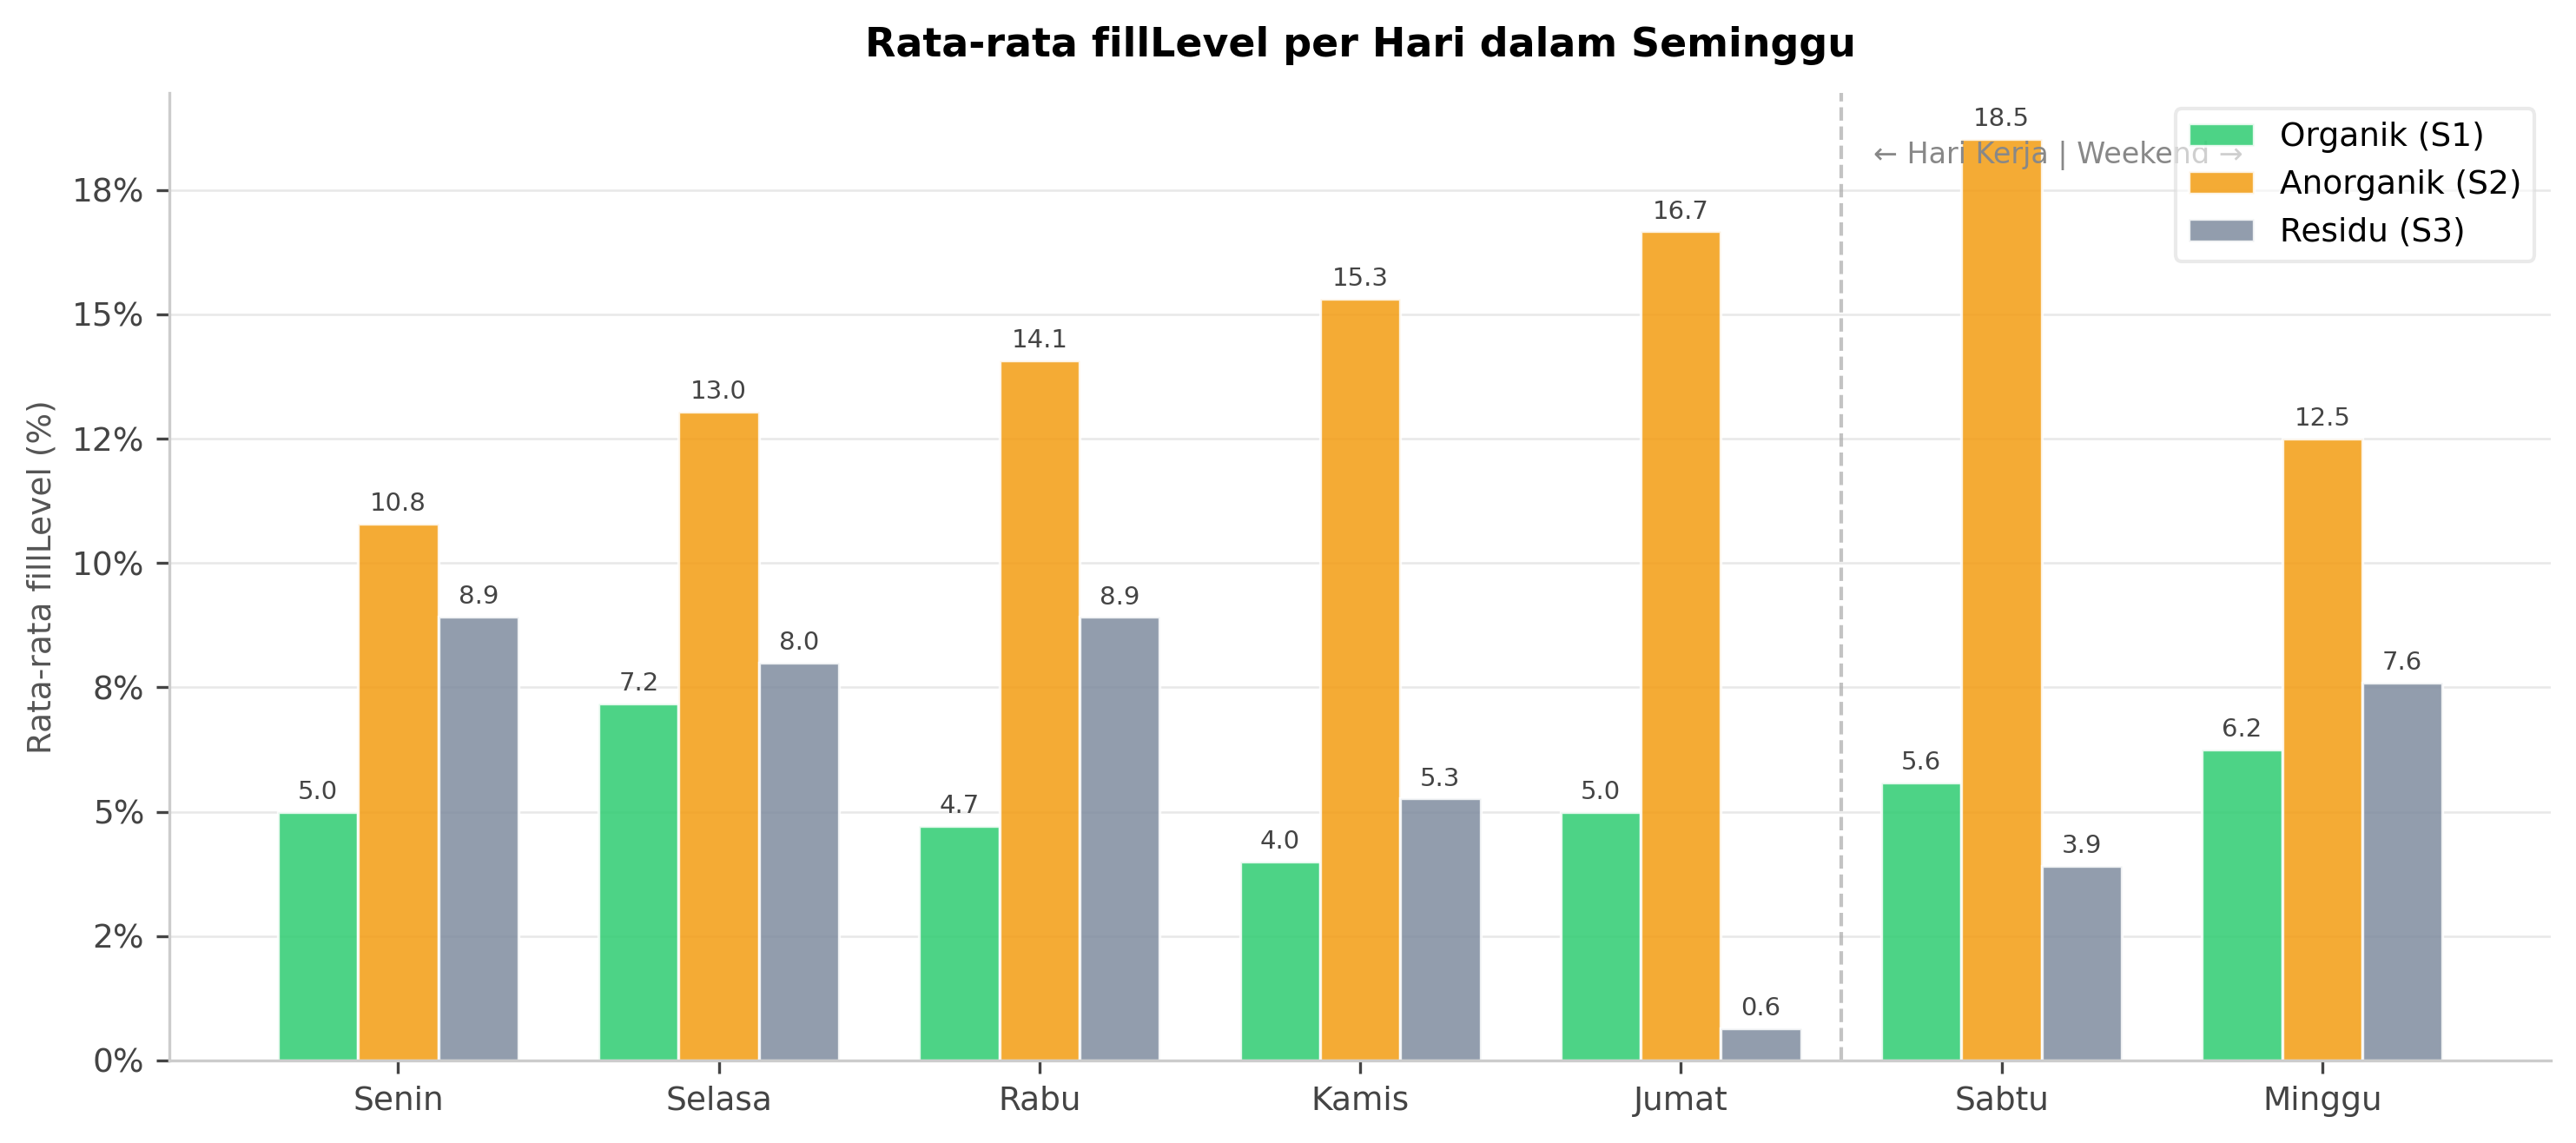
\includegraphics[width=\textwidth]{images/pola-mingguan.png}
  % RENAME: image17.png → pola-mingguan.png
\end{figure}

Rata-rata hari kerja: 5,2\% (Organik), 14,0\% (Anorganik), 6,3\% (Residu). Rata-rata \textit{weekend}: 5,9\% (Organik), 15,6\% (Anorganik), 5,8\% (Residu). Perbedaan antar hari kerja dan \textit{weekend} tidak signifikan karena \textit{fillLevel} bersifat kumulatif, sehingga nilai tinggi pada hari tertentu dapat mencerminkan akumulasi dari hari-hari sebelumnya sebelum terjadi pengosongan.

\subsubsection{Analisis Pengaruh Hari Libur}

Tabel \ref{tab:pola-libur} menyajikan rata-rata \textit{fillLevel} berdasarkan kategori hari, dan Gambar \ref{fig:pola-libur} memvisualisasikan perbandingannya.

\begin{table}[H]
  \caption{Pola Hari Libur}
  \label{tab:pola-libur}
  \centering
  \begin{tabular}{| l | l | l | l | l |}
    \hline
    \textbf{Kategori Hari} & \textbf{Organik} & \textbf{Anorganik} & \textbf{Residu} & \textbf{Jumlah Hari} \\
    \hline
    Hari kerja (Senin--Jumat) & 5,1\%  & 13,6\% & 6,9\% & 24 hari \\
    \hline
    \textit{Weekend} (Sabtu--Minggu) & 5,9\% & 15,6\% & 5,8\% & 10 hari \\
    \hline
    Hari libur nasional & 5,5\% & 18,0\% & 3,5\% & 3 hari \\
    \hline
  \end{tabular}
\end{table}

\begin{figure}[H]
  \caption{Rata-rata \textit{fillLevel} Berdasarkan Kategori Hari}
  \label{fig:pola-libur}
  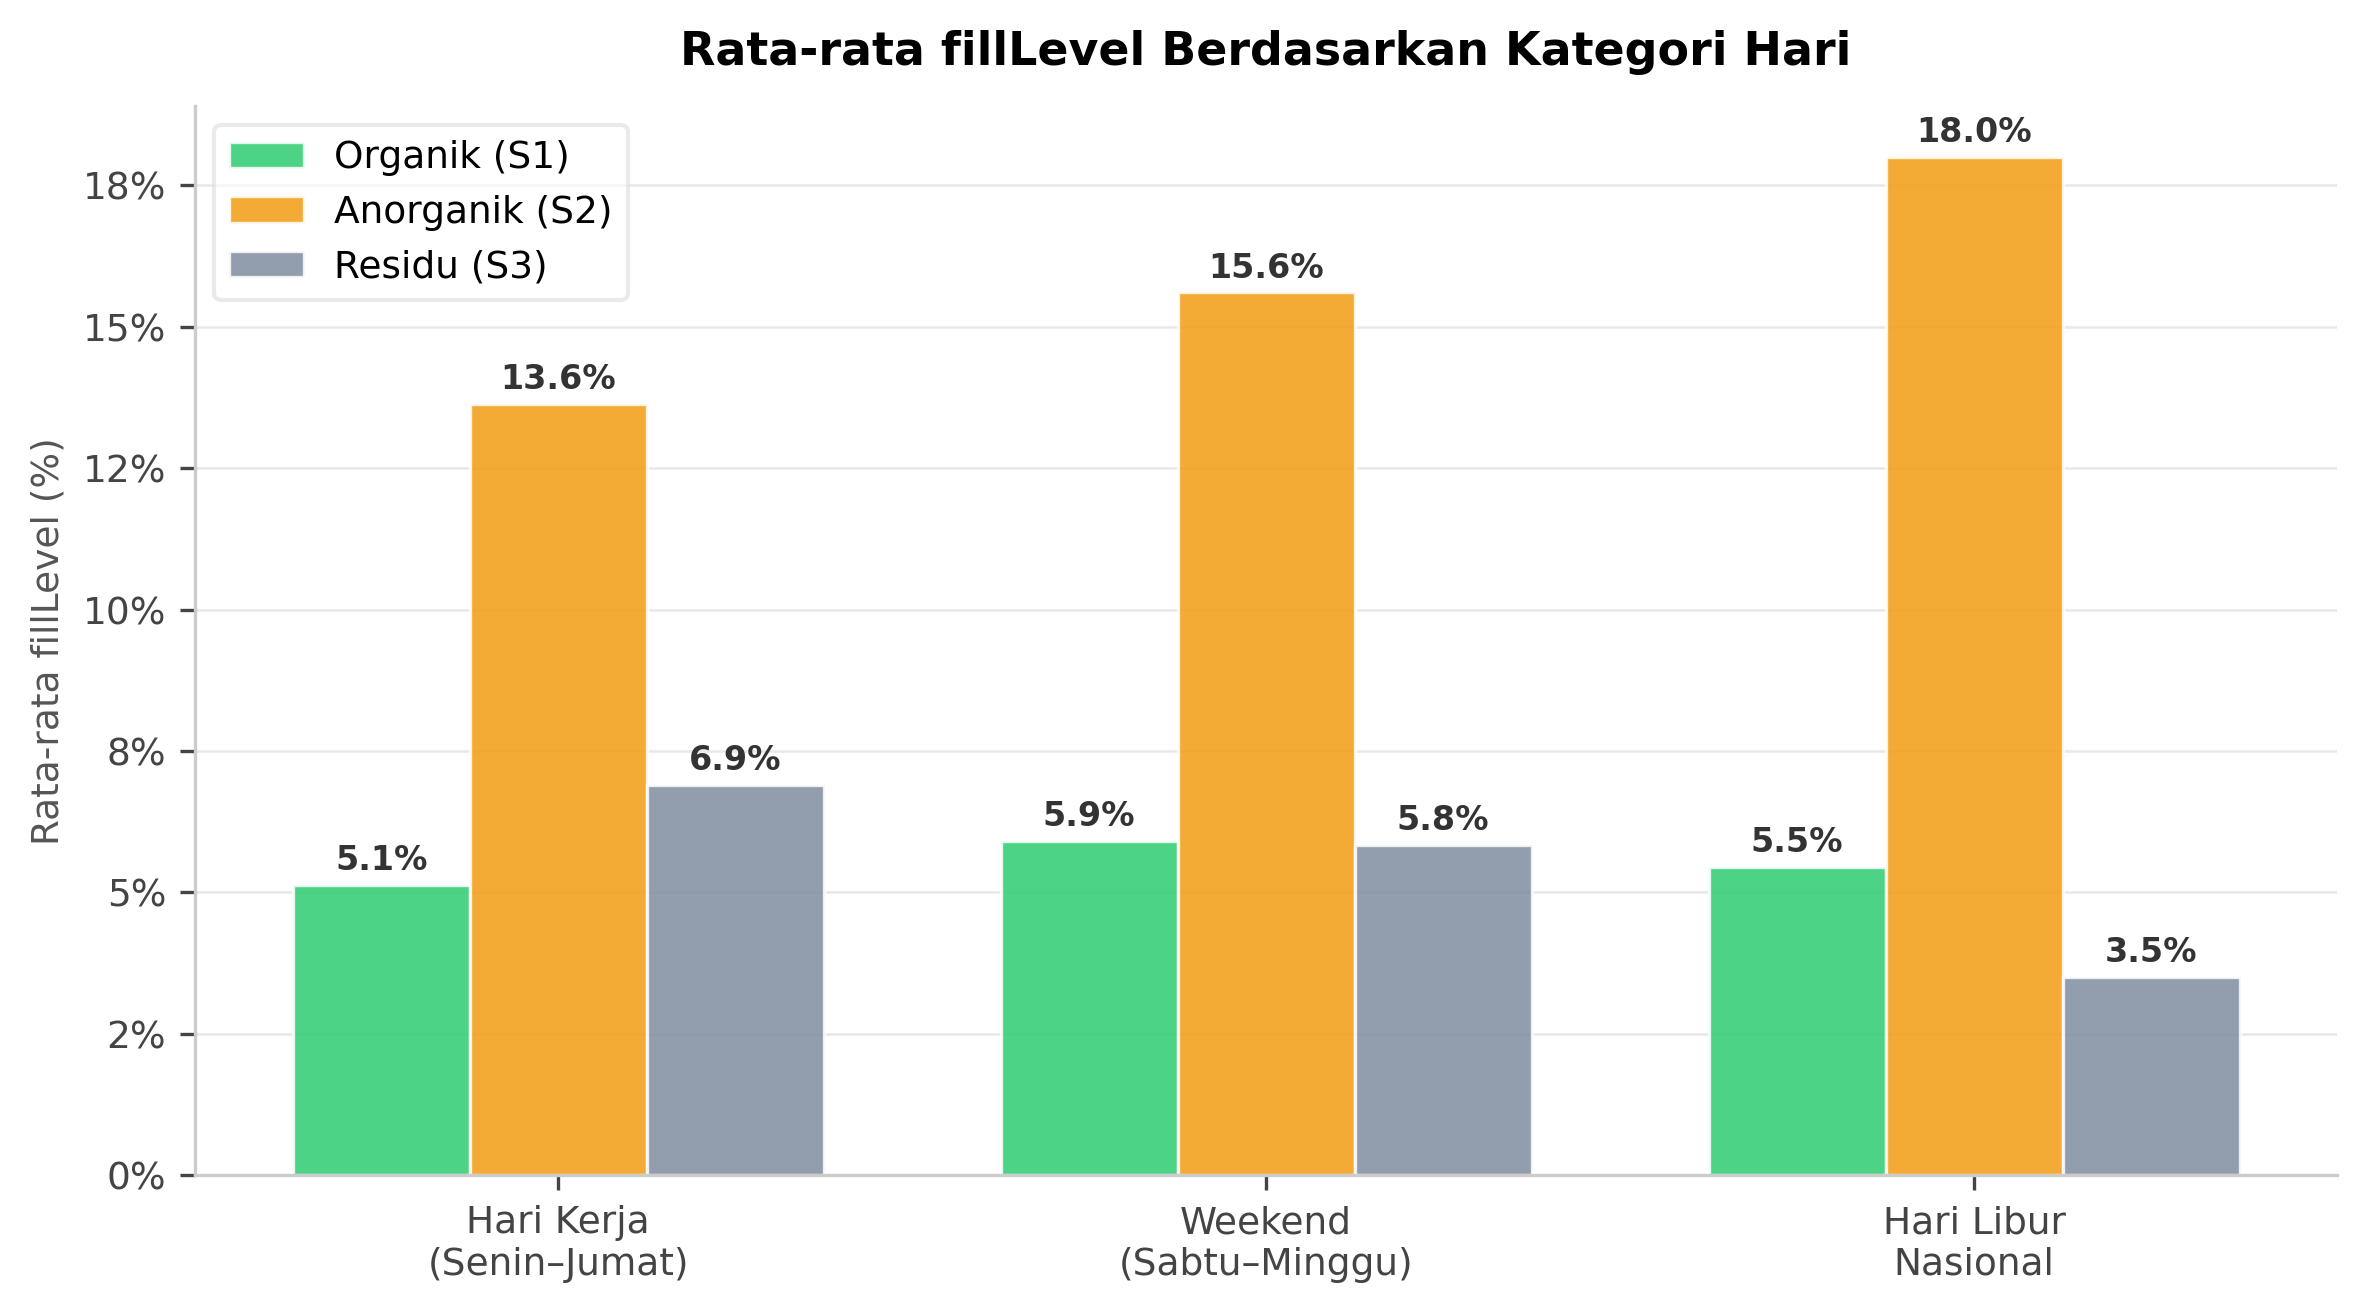
\includegraphics[width=0.8\textwidth]{images/pola-libur.png}
  % RENAME: image18.png → pola-libur.png
\end{figure}

Hari libur nasional yang memiliki data dalam periode pengumpulan meliputi 25 sampai 26 Desember 2025 (Natal) dan 1 Januari 2026 (Tahun Baru). Tingginya rata-rata \textit{fillLevel} Anorganik pada hari libur (18,0\%) merupakan efek akumulasi kumulatif, yaitu tempat sampah yang tidak dikosongkan saat libur membawa nilai \textit{fillLevel} dari hari-hari sebelumnya, bukan mencerminkan aktivitas pembuangan yang lebih tinggi.

\subsubsection{Analisis Penambahan (Delta)}

Analisis delta mengidentifikasi frekuensi dan waktu terjadinya penambahan sampah yang sesungguhnya. Tabel \ref{tab:analisis-delta} menyajikan proporsi jenis perubahan \textit{fillLevel}.

\begin{table}[H]
  \caption{Analisis Delta \textit{fillLevel}}
  \label{tab:analisis-delta}
  \centering
  \begin{tabular}{| l | l | l | l |}
    \hline
    \textbf{Jenis Perubahan} & \textbf{Organik} & \textbf{Anorganik} & \textbf{Residu} \\
    \hline
    Tidak ada perubahan ($\delta$ = 0)         & 95,5\% & 93,4\% & 94,2\% \\
    \hline
    Penambahan kecil (+10\%)                   & 2,4\%  & 3,8\%  & 3,1\% \\
    \hline
    Penambahan besar (+20\% atau lebih)        & 0\%    & 0,7\%  & 0\% \\
    \hline
    Pengurangan / dikosongkan ($\delta$ $<$ 0) & 2,1\%  & 2,1\%  & 2,7\% \\
    \hline
  \end{tabular}
\end{table}

Tabel \ref{tab:delta-perjam} menyajikan distribusi temporal \textit{event} penambahan berdasarkan rentang jam.

\begin{table}[H]
  \caption{Distribusi \textit{Event} Penambahan per Rentang Jam}
  \label{tab:delta-perjam}
  \centering
  \begin{tabular}{| l | l | l | l | l | l |}
    \hline
    \textbf{Rentang Jam} & \textbf{S1} & \textbf{S2} & \textbf{S3} & \textbf{Total} & \textbf{\% dari 27} \\
    \hline
    07:00--09:00 & 2 & 2 & 1 & 5  & 18,5\% \\
    \hline
    09:00--12:00 & 1 & 2 & 3 & 6  & 22,2\% \\
    \hline
    12:00--14:00 & 0 & 3 & 2 & 5  & 18,5\% \\
    \hline
    14:00--17:00 & 3 & 4 & 1 & 8  & 29,6\% \\
    \hline
    17:00--19:00 & 1 & 2 & 0 & 3  & 11,1\% \\
    \hline
    19:00--07:00 & 0 & 0 & 0 & 0  & 0\% \\
    \hline
    \textbf{Total} & \textbf{7} & \textbf{13} & \textbf{7} & \textbf{27} & \textbf{100\%} \\
    \hline
  \end{tabular}
\end{table}

\begin{figure}[H]
  \caption{Distribusi Kategori Delta dan \textit{Event} Penambahan per Rentang Jam}
  \label{fig:distribusi-delta}
  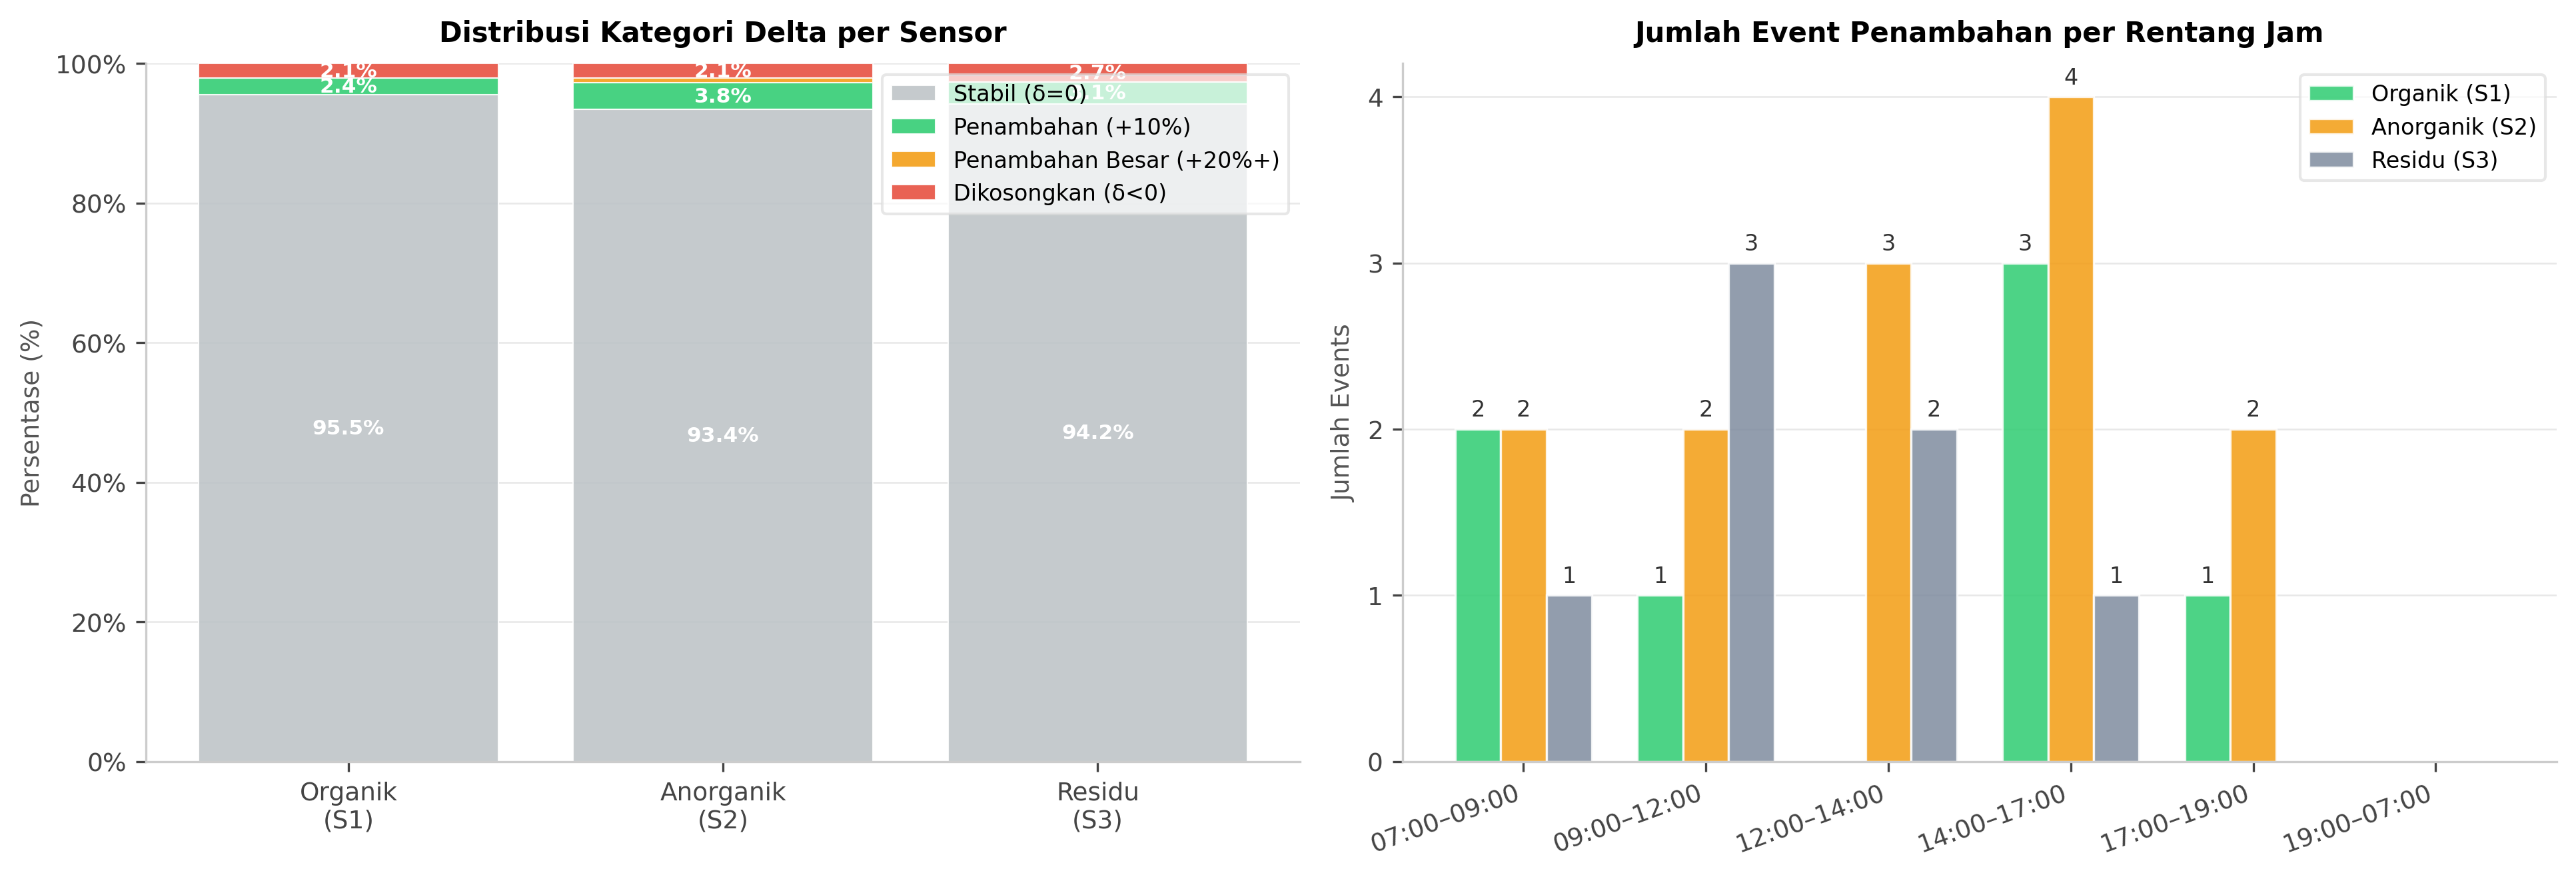
\includegraphics[width=\textwidth]{images/distribusi-delta.png}
  % RENAME: image19.png → distribusi-delta.png
\end{figure}

Total 27 \textit{event} penambahan terdeteksi selama periode observasi, dengan distribusi temporal divisualisasikan pada Gambar \ref{fig:distribusi-delta}. Penambahan terbanyak terjadi pada rentang 14:00--17:00 (29,6\%), diikuti 09:00--12:00 (22,2\%). Tidak ada penambahan yang terdeteksi pada malam hari (19:00--07:00), konsisten dengan tidak adanya aktivitas kampus.

\subsubsection{Analisis Komposisi Jenis Sampah}

Tabel \ref{tab:pola-jenis} menyajikan perbandingan pola pembuangan antar jenis sampah.

\begin{table}[H]
  \caption{Pola Setiap Jenis Sampah}
  \label{tab:pola-jenis}
  \begin{tabularx}{\textwidth}{| X | l | l | l |}
    \hline
    \textbf{Aspek} & \textbf{Organik (S1)} & \textbf{Anorganik (S2)} & \textbf{Residu (S3)} \\
    \hline
    Rata-rata \textit{fillLevel}          & 5,3\%    & 14,4\%    & 6,4\% \\
    \hline
    Max \textit{fillLevel} tercatat       & 20\%     & 40\%      & 20\% \\
    \hline
    Frekuensi penambahan                  & 2,4\%    & 4,5\%     & 3,1\% \\
    \hline
    Jumlah \textit{event} penambahan      & 7        & 13        & 7 \\
    \hline
    Total delta positif                   & +70\%    & +150\%    & +70\% \\
    \hline
    Korelasi dengan hari kerja            & Tinggi   & Sangat Tinggi & Tinggi \\
    \hline
  \end{tabularx}
\end{table}

\begin{figure}[H]
  \caption{Perbandingan Pola Jenis Sampah}
  \label{fig:perbandingan-jenis}
  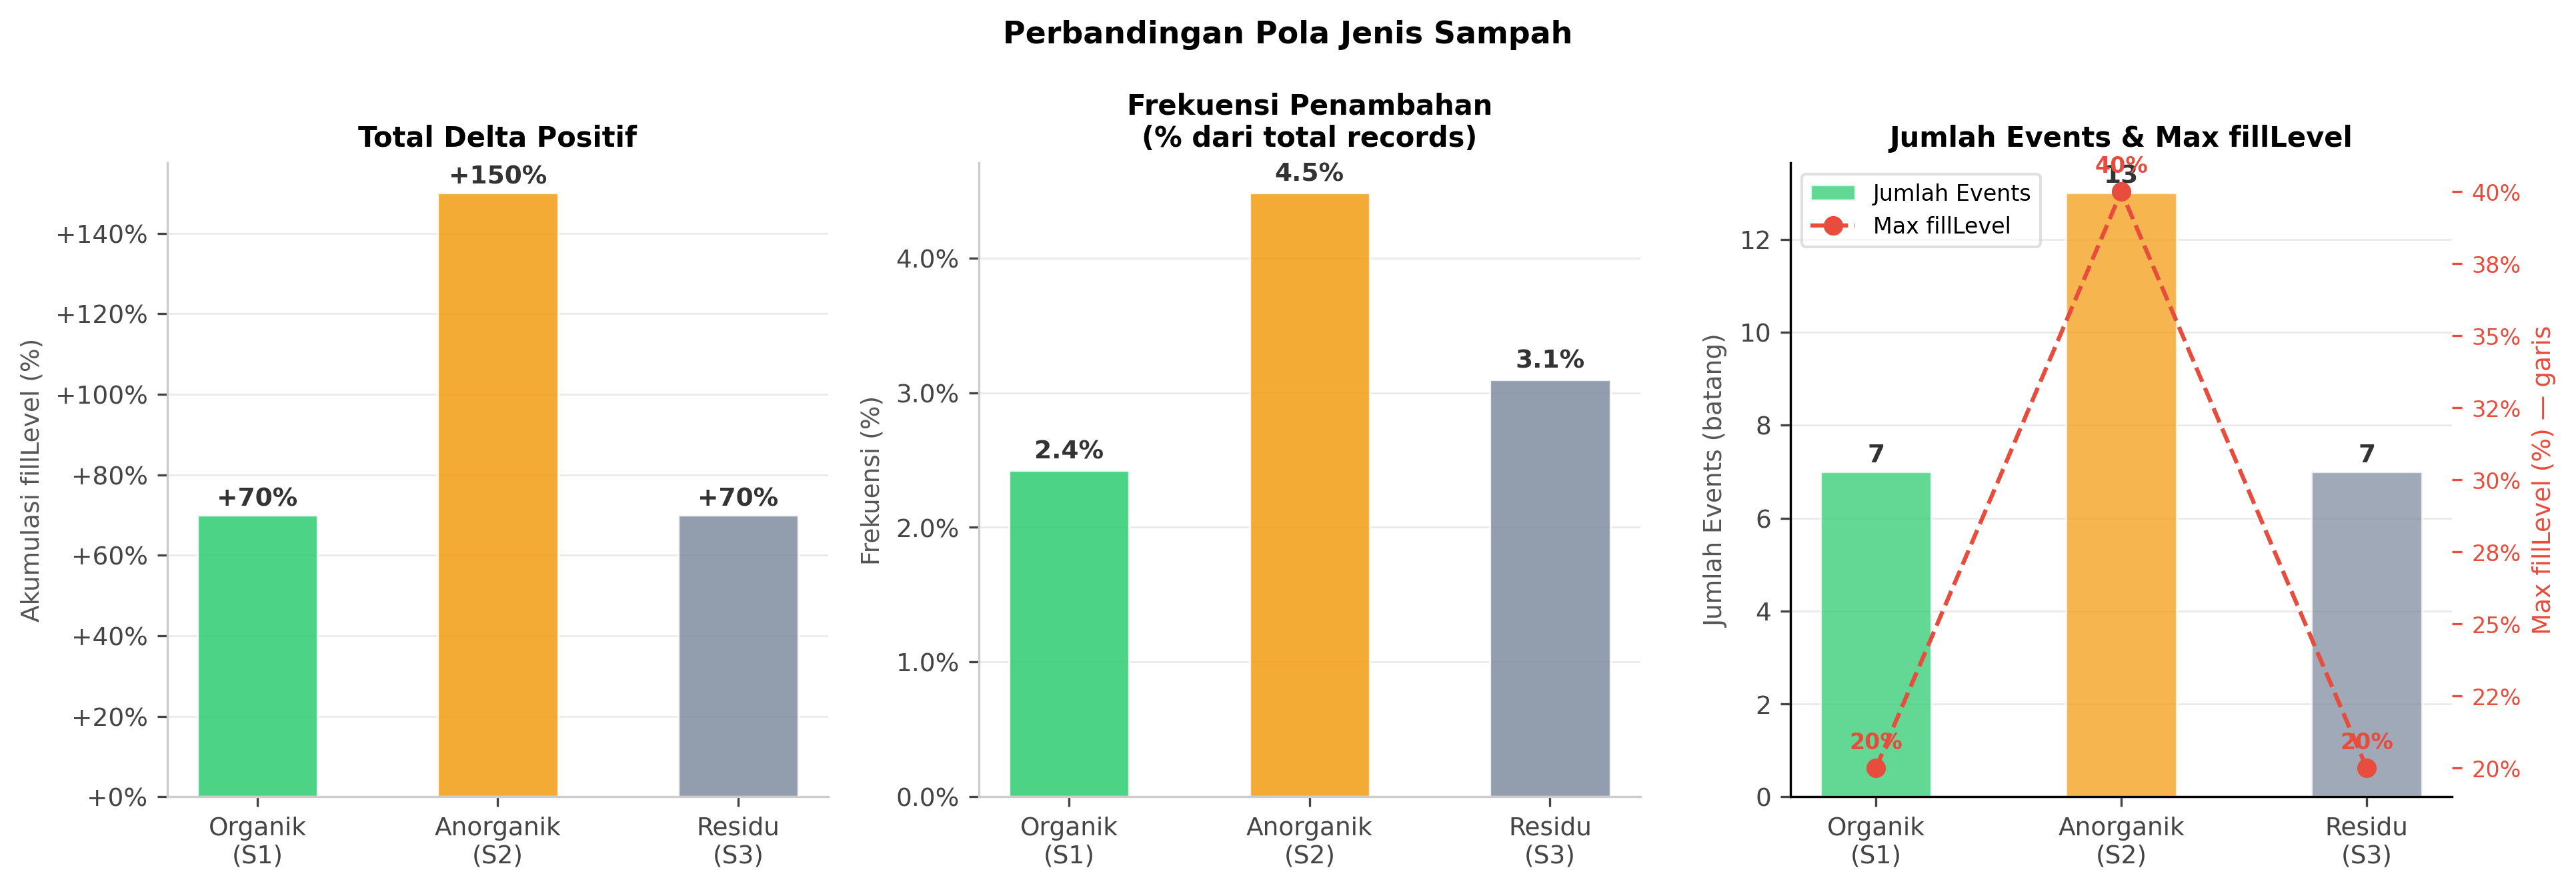
\includegraphics[width=\textwidth]{images/perbandingan-jenis.png}
  % RENAME: image20.png → perbandingan-jenis.png
\end{figure}

Sampah Anorganik memiliki volume dan frekuensi penambahan tertinggi (51,7\% dari total delta), sebagaimana divisualisasikan pada Gambar \ref{fig:perbandingan-jenis}. Organik dan Residu masing-masing berkontribusi 24,1\%. Hal ini sesuai dengan karakteristik lokasi sebagai area laboratorium yang menghasilkan lebih banyak sampah plastik, kertas, dan kemasan.

\subsubsection{Analisis Ketepatan Klasifikasi Sampah}

Selain analisis volume, dilakukan juga observasi terhadap ketepatan klasifikasi sampah oleh pengguna. Observasi visual dilakukan pada beberapa waktu \textit{sampling} untuk mengidentifikasi sampah yang dibuang pada kategori yang tidak sesuai peruntukannya (lihat Lampiran C). Berdasarkan dokumentasi foto yang tersedia, temuan observasi ketepatan klasifikasi disajikan pada Tabel \ref{tab:kesesuaian-jenis}.

\begin{table}[H]
  \caption{Kesesuaian Jenis Sampah}
  \label{tab:kesesuaian-jenis}
  \begin{tabularx}{\textwidth}{| l | X | l |}
    \hline
    \textbf{Tempat Sampah} & \textbf{Temuan} & \textbf{Validasi Lapangan} \\
    \hline
    Organik (Hijau) & Ditemukan kantong plastik dan sisa bungkus makanan & Terdokumentasi foto (Lampiran C) \\
    \hline
    Anorganik (Kuning) & Ditemukan beberapa sisa tisu basah yang seharusnya masuk ke residu & Terdokumentasi foto (Lampiran C) \\
    \hline
    Residu (Hitam) & Ditemukan sisa makanan dalam wadah dan tisu bekas & Terdokumentasi foto (Lampiran C) \\
    \hline
  \end{tabularx}
\end{table}

Temuan utama dari observasi ketepatan klasifikasi adalah sebagai berikut.

\begin{enumerate}
  \item \textbf{Plastik di Tempat Sampah Organik.} Ditemukan plastik kemasan makanan di tempat sampah organik. Pengguna cenderung membuang kemasan makanan beserta sisa makanannya sekaligus karena dianggap satu kesatuan.

  \item \textbf{Residu di Tempat Sampah Anorganik.} Ditemukan sampah yang seharusnya masuk kategori residu seperti tisu kotor dan \textit{styrofoam} di tempat sampah anorganik, kemungkinan karena kurangnya pemahaman tentang definisi sampah residu.

  \item \textbf{Campuran di Tempat Sampah Residu.} Tempat sampah residu ditemukan mengandung sisa makanan yang seharusnya masuk kategori organik. Hal ini mengindikasikan bahwa pengguna mengalami kebingungan dalam mengidentifikasi kategori residu, yang memang memiliki definisi paling tidak intuitif dibandingkan kategori organik dan anorganik.
\end{enumerate}

Temuan ini menunjukkan perlunya sosialisasi berkala tentang jenis sampah dan penyediaan infografis panduan singkat di dekat lokasi tempat sampah untuk meningkatkan ketepatan klasifikasi oleh pengguna.

\subsubsection{Sintesis Temuan Analisis}
\label{sec:sintesis-temuan}

Seluruh analisis pada subbab ini dilakukan menggunakan pendekatan \textit{analisis deskriptif}, yaitu pendekatan yang bertujuan mendeskripsikan dan merangkum karakteristik suatu fenomena berdasarkan data, tanpa melakukan inferensi kausal maupun prediksi \autocite{loeb2017descriptive}. Pendekatan ini dipilih karena tujuan penelitian adalah mengidentifikasi dan mengkarakterisasi pola pembuangan yang terjadi, bukan memodelkan atau memprediksinya. Analisis deskriptif terhadap data deret waktu (\textit{time series}) yang dikumpulkan mencakup peringkasan statistik, agregasi temporal, dan visualisasi untuk mengungkap struktur dalam data \autocite{wickham2016r}.

Berdasarkan analisis deskriptif yang dilakukan, penelitian ini mengidentifikasi empat pola pembuangan sampah. Sebuah pola didefinisikan sebagai keteraturan yang konsisten muncul dalam data sepanjang periode pengamatan, bukan kejadian tunggal yang bersifat acak. Keempat pola ini dibedakan menjadi dua jenis berdasarkan dimensi analisisnya, yaitu tiga \textbf{pola temporal} (keteraturan pada dimensi waktu) dan satu \textbf{pola komposisi} (keteraturan pada dimensi jenis sampah). Setiap pola diberi nama yang jelas sebagai identitasnya. Tabel \ref{tab:sintesis-temuan} merangkum keempat pola tersebut beserta klasifikasinya.

\begin{table}[H]
  \caption{Sintesis dan Klasifikasi Pola Pembuangan Sampah}
  \label{tab:sintesis-temuan}
  \begin{tabularx}{\textwidth}{| l | l | X |}
    \hline
    \textbf{Nama Pola} & \textbf{Jenis} & \textbf{Deskripsi Kuantitatif} \\
    \hline
    Pola \textit{Peak Hour} & Pola Temporal & Puncak penambahan pada pukul 14:00--17:00 (8 dari 27 \textit{event}, 29,6\%) \\
    \hline
    Pola Konsentrasi Jam Aktif & Pola Temporal & Seluruh \textit{event} terjadi pada rentang 07:00--19:00 di hari kerja \\
    \hline
    Pola Pengaruh Hari Libur & Pola Temporal & Aktivitas penambahan turun hingga nol pada hari libur nasional \\
    \hline
    Pola Dominasi Anorganik & Pola Komposisi & Sampah anorganik menyumbang 13 dari 27 \textit{event} (48,1\%) dan 51,7\% volume delta positif \\
    \hline
  \end{tabularx}
\end{table}

Ketiga pola temporal, yaitu Pola \textit{Peak Hour}, Pola Konsentrasi Jam Aktif, dan Pola Pengaruh Hari Libur, merupakan keteraturan yang muncul pada dimensi waktu dan saling melengkapi dalam menggambarkan kapan aktivitas pembuangan terjadi. Sementara itu, Pola Dominasi Anorganik merupakan keteraturan pada dimensi komposisi jenis sampah, yang konsisten muncul sepanjang periode pengamatan (bukan fluktuasi acak), sehingga sah dikategorikan sebagai pola meskipun tidak berdimensi waktu. Keempat pola ini telah divalidasi kewajarannya terhadap observasi lapangan dan konsisten dengan karakteristik aktivitas di lokasi penelitian, serta secara bersama-sama menjawab RM-2.

\subsection{Hasil Evaluasi Adaptasi \textit{Firmware} (SE-04)}

Skenario SE-04 mengevaluasi efektivitas adaptasi \textit{firmware} yang dilakukan terhadap perangkat \textit{Smart Waste Bin}. Evaluasi ini merupakan bagian dari penilaian keberhasilan rancangan dan implementasi sistem (RM-1), khususnya untuk menilai sejauh mana adaptasi \textit{firmware} meningkatkan keandalan operasional dan kualitas data yang dikumpulkan sistem.

Tabel \ref{tab:hasil-firmware} menyajikan hasil evaluasi untuk setiap adaptasi \textit{firmware}.

\begin{table}[H]
  \caption{Hasil Evaluasi Adaptasi \textit{Firmware}}
  \label{tab:hasil-firmware}
  \begin{tabularx}{\textwidth}{| X | X | X | l |}
    \hline
    \textbf{Peningkatan} & \textbf{Masalah yang Diatasi} & \textbf{Hasil Evaluasi} & \textbf{Status} \\
    \hline
    Perubahan interval (8 jam → 2,5 jam) & Resolusi data terlalu rendah untuk analisis pola temporal & 8--9 data \textit{points} per hari, pola harian berhasil teridentifikasi & Efektif \\
    \hline
    \textit{Median filter} (5 \textit{readings}) & \textit{Noise} pada pembacaan sensor & \textit{fillLevel} stabil tanpa lompatan acak & Efektif \\
    \hline
    \textit{Auto-recovery mechanism} & Sensor \textit{hang} menyebabkan \textit{data loss} & Tidak ada kejadian \textit{hang} setelah implementasi & Efektif \\
    \hline
    \textit{Warm-up readings} & Pembacaan awal tidak stabil & Pembacaan pertama lebih konsisten & Efektif \\
    \hline
    GPIO \textit{isolation} & \textit{Floating state} saat \textit{sleep} & Konsumsi daya tidak berubah signifikan & Tidak Efektif \\
    \hline
  \end{tabularx}
\end{table}

Dari lima adaptasi \textit{firmware} yang diimplementasikan, empat menunjukkan efektivitas. Perubahan interval pengambilan data menjadi fondasi keberhasilan analisis pola. \textit{Median filter} berhasil mereduksi \textit{noise} selama periode pengujian. Mekanisme \textit{auto-recovery} terbukti efektif karena sebelum implementasi, sensor pernah mengalami kondisi \textit{hang} dan tidak mengirim data meskipun baterai masih baik, namun setelah \textit{firmware} baru di-\textit{upload}, kejadian tersebut tidak terulang. Satu adaptasi yang tidak efektif adalah GPIO \textit{isolation}, kemungkinan karena konsumsi daya utama berasal dari modul GSM SIM800L yang tidak terpengaruh oleh isolasi GPIO.

% ============================================================
\section{Pemenuhan Kebutuhan Sistem}
\label{sec:pemenuhan-kebutuhan}
% ============================================================

Subbab ini menyajikan evaluasi pemenuhan kebutuhan fungsional dan nonfungsional yang telah diidentifikasi pada Bab III, berdasarkan hasil pengujian pada Subbab \ref{sec:hasil-evaluasi}.

\subsection{Pemenuhan Kebutuhan Fungsional}

Tabel \ref{tab:pemenuhan-kf-hasil} menyajikan evaluasi pemenuhan seluruh kebutuhan fungsional.

\begin{table}[H]
  \caption{Pemenuhan Kebutuhan Fungsional}
  \label{tab:pemenuhan-kf-hasil}
  \begin{tabularx}{\textwidth}{| l | X | X | l |}
    \hline
    \textbf{ID} & \textbf{Kebutuhan Fungsional} & \textbf{Bukti Pemenuhan} & \textbf{Status} \\
    \hline
    KF-01 & Pembacaan tingkat kepenuhan & Sensor VL53L0X membaca jarak dan mengkonversi ke \textit{fillLevel} & Terpenuhi \\
    \hline
    KF-02 & Transmisi data otomatis periodik & Data terkirim setiap $\sim$2,5 jam via MQTT & Terpenuhi \\
    \hline
    KF-03 & \textit{Timestamp} dan \textit{identifier} & Setiap \textit{record} memiliki \textit{timestamp} dan \texttt{sensor\_id} & Terpenuhi \\
    \hline
    KF-04 & Konversi jarak ke persentase & \textit{Firmware} mengkonversi mm ke \% menggunakan rumus konversi & Terpenuhi \\
    \hline
    KF-05 & Penyimpanan data ke \textit{database} & Data tersimpan di Supabase PostgreSQL & Terpenuhi \\
    \hline
    KF-06 & \textit{Query} data berdasarkan \textit{filter} & API mendukung \textit{filter} \texttt{sensorId} dan \texttt{timerange} & Terpenuhi \\
    \hline
    KF-07 & Analisis pola temporal & Pola harian, mingguan, dan libur teridentifikasi & Terpenuhi \\
    \hline
    KF-08 & Statistik deskriptif & \textit{Mean}, median, std dev dihitung per sensor & Terpenuhi \\
    \hline
    KF-09 & Visualisasi data \textit{dashboard} & \textit{Dashboard} menampilkan \textit{chart} dan status terkini & Terpenuhi \\
    \hline
    KF-10 & Grafik pola temporal & \textit{Line chart} menampilkan tren \textit{fillLevel} & Terpenuhi \\
    \hline
  \end{tabularx}
\end{table}

Seluruh kebutuhan fungsional (KF-01 sampai KF-10) berhasil dipenuhi oleh sistem yang diimplementasikan.

\subsection{Pemenuhan Kebutuhan Nonfungsional}

Tabel \ref{tab:pemenuhan-knf-hasil} menyajikan evaluasi pemenuhan kebutuhan nonfungsional.

\begin{table}[H]
  \caption{Pemenuhan Kebutuhan Nonfungsional}
  \label{tab:pemenuhan-knf-hasil}
  \begin{tabularx}{\textwidth}{| l | X | l | l | l | l |}
    \hline
    \textbf{ID} & \textbf{Kebutuhan} & \textbf{Target} & \textbf{Aktual} & \textbf{Kategori} & \textbf{Status} \\
    \hline
    KNF-01 & Waktu pembacaan sensor       & $<$ 1 menit & $<$ 5 detik & \textit{Performance} & Terpenuhi \\
    \hline
    KNF-02 & Latensi transmisi data       & $<$ 10 detik & $<$ 3 detik & \textit{Performance} & Terpenuhi \\
    \hline
    KNF-03 & \textit{Response time dashboard} & $<$ 3 detik & $<$ 1 detik & \textit{Performance} & Terpenuhi \\
    \hline
    KNF-04 & Waktu \textit{query database} & $<$ 5 detik & $<$ 500 ms & \textit{Performance} & Terpenuhi \\
    \hline
    KNF-05 & \textit{Uptime} sistem IoT   & $>$ 95\% & 91,9\% & \textit{Reliability} & Sebagian \\
    \hline
    KNF-06 & Konsistensi interval         & $\pm$15 menit & $\pm$12 menit* & \textit{Reliability} & Terpenuhi \\
    \hline
    KNF-07 & Kelengkapan data             & $>$ 90\% & 91,9\% & \textit{Reliability} & Terpenuhi \\
    \hline
    KNF-08 & Akurasi sensor \textit{fillLevel} & $<$ 10\% \textit{error} & Sesuai & \textit{Accuracy} & Terpenuhi \\
    \hline
  \end{tabularx}
\end{table}

*KNF-06 dihitung berdasarkan Sensor 1 dan 2. Sensor 3 memiliki std dev 38 menit yang melebihi toleransi akibat anomali konsumsi daya.

KNF-05 dan KNF-07 menggunakan metrik yang sama (91,9\%) namun berstatus berbeda karena \textit{threshold} yang berbeda. KNF-05 menargetkan 95\% sehingga berstatus sebagian, sedangkan KNF-07 menargetkan 90\% sehingga terpenuhi. Dari 8 kebutuhan nonfungsional, 7 berhasil dipenuhi sepenuhnya dan 1 kebutuhan (KNF-05) dipenuhi sebagian karena faktor eksternal berupa \textit{broker} MQTT vendor yang dimatikan dan baterai bocor.

% ============================================================
\section{Diskusi Hasil Evaluasi}
\label{sec:diskusi-evaluasi}
% ============================================================

\subsection{Analisis Konsumsi Daya pada Sensor 3}

Sensor 3 (Residu) menunjukkan anomali berupa konsumsi arus hampir dua kali lipat (210--235 mA) dibandingkan Sensor 1 dan 2 (110--140 mA), meskipun ketiga unit menggunakan spesifikasi komponen identik dan \textit{firmware} yang sama. Anomali ini menyebabkan baterai Sensor 3 lebih cepat habis dan mengakibatkan \textit{data loss} lebih tinggi (23,6\%) dibandingkan sensor lainnya ($\sim$2\%).

Berbagai upaya optimasi \textit{firmware} telah dilakukan termasuk GPIO \textit{isolation} dan optimasi urutan \textit{shutdown}, namun konsumsi daya tetap tinggi. Ini mengindikasikan akar masalah bukan pada \textit{software} melainkan \textit{hardware}. Beberapa hipotesis penyebab: komponen pasif yang rusak atau tidak terpasang dengan benar, \textit{short circuit} ringan pada PCB, variasi karakteristik komponen aktif seperti modul SIM800L, atau kerusakan pada jalur \textit{power} akibat proses \textit{assembly}.

Temuan ini menunjukkan pentingnya \textit{quality control} dan \textit{burn-in testing} sebelum \textit{deployment} perangkat IoT. Untuk produksi massal, disarankan menetapkan batas toleransi konsumsi daya dan melakukan \textit{reject} pada unit yang melebihi batas tersebut.

\subsection{Validitas Temuan}

Untuk memastikan validitas pola yang teridentifikasi, dilakukan triangulasi dengan observasi kontekstual lapangan berdasarkan pengetahuan kondisi aktual lokasi penelitian dan dokumentasi foto (Lampiran C). Tabel \ref{tab:validasi-pola} menyajikan validasi setiap pola terhadap kondisi aktual di lapangan.

\begin{table}[H]
  \caption{Validasi Pola dengan Observasi Lapangan}
  \label{tab:validasi-pola}
  \begin{tabularx}{\textwidth}{| l | X | X | X |}
    \hline
    \textbf{No} & \textbf{Pola Teridentifikasi} & \textbf{Evidensi Data} & \textbf{Validasi Lapangan} \\
    \hline
    1 & \textit{Peak hour} pada pukul 14:00--17:00 & 8 \textit{event} penambahan terdeteksi pada rentang ini, tertinggi dari semua rentang (29,6\% dari 27 \textit{event}) & Konsisten dengan jadwal aktivitas lab; warga lab umumnya membuang sampah setelah sesi kerja siang \\
    \hline
    2 & Aktivitas pembuangan pada hari kerja lebih tinggi & Seluruh 27 \textit{event} penambahan terjadi pada jam aktif kampus 07:00--19:00, tidak ada penambahan pada malam hari dan \textit{weekend} & Dikonfirmasi; Lab IoT tidak beroperasi di luar jam kerja dan akses terbatas \\
    \hline
    3 & Aktivitas pembuangan turun drastis pada hari libur nasional & Tidak ada \textit{event} penambahan terdeteksi pada hari libur; \textit{fillLevel} Anorganik tinggi (18,0\%) merupakan efek akumulasi kumulatif & Dikonfirmasi; gedung tidak beroperasi pada 25--26 Des dan 1 Jan \\
    \hline
    4 & Dominasi sampah anorganik (51,7\% dari total volume) & Anorganik menyumbang +150\% delta positif dari total +290\%, setara 51,7\% dari total \textit{event} penambahan (13 dari 27) & Konsisten dengan observasi; pengguna lab menghasilkan kemasan minuman dan makanan lebih banyak \\
    \hline
  \end{tabularx}
\end{table}

Seluruh pola utama tervalidasi melalui observasi lapangan, meningkatkan \textit{confidence} bahwa pola-pola yang teridentifikasi mencerminkan kondisi aktual, bukan artefak dari keterbatasan sensor atau \textit{noise} data.

\subsection{Implikasi Praktis Pengelolaan Sampah}

Temuan penelitian ini memiliki beberapa implikasi praktis untuk pengelolaan sampah di lingkungan kampus.

\begin{enumerate}
  \item Berdasarkan pola \textit{peak hour}, jadwal pengosongan tempat sampah dapat difokuskan pada sore hari kerja (setelah pukul 14:00), bukan pagi hari atau \textit{weekend}, untuk efisiensi operasional.

  \item Dominasi sampah anorganik (51,7\%) menunjukkan potensi program pengurangan kemasan sekali pakai atau penyediaan fasilitas \textit{refill} untuk menekan volume sampah.

  \item Empat dari lima adaptasi \textit{firmware} yang telah diuji dapat direkomendasikan untuk diadopsi pada perangkat \textit{Smart Waste Bin} di lingkungan dengan aktivitas terkonsentrasi pada jam-jam tertentu.

  \item Sistem Pemantauan Sampah Berbasis \textit{Internet of Things} memberikan data objektif untuk pengambilan keputusan pengelolaan sampah, menggantikan estimasi manual yang subjektif dan tidak terstruktur.
\end{enumerate}